\section{Điểm, đường thẳng và mặt phẳng trong không gian}
\subsection{Tóm tắt lí thuyết}
\subsubsection{Khái niệm mở đầu}
\begin{enumerate}
	\item Để biểu diễn một mặt phẳng ta thường dùng hình bình hành hay một miền góc.\\ Để kí hiệu mặt phẳng ta dùng chữ cái in hoa hoặc chữ cái Hi Lạp đặt trong dấu ngoặc đơn.\\ Ví dụ: mặt phẳng $(P)$, mặt phẳng $(\alpha)$ hoặc viết tắt là mp$(P)$, mp$(\alpha)$ hoặc $(P)$, $(\alpha)$, \ldots
	\begin{center}
		\begin{tikzpicture}[declare function={a=4;}]
		% Các điểm của tứ giác
		\coordinate (A) at (0,0);
		\coordinate (B) at (a,0);
		\coordinate (C) at ($(B)+(50:{a/2})$);
		\coordinate (D) at ($(C)+(-a,0)$);
		
		% Vẽ tứ giác
		\draw (A) -- (B) -- (C) -- (D) -- cycle;
		
		% Vẽ ký hiệu góc tại điểm A
		\draw pic[draw, angle radius=6mm, "$P$"]{angle=B--A--D};
		
		\end{tikzpicture}
		\begin{tikzpicture}[declare function={a=4;}]
		% Các điểm của tứ giác
		\coordinate (A) at (0,0);
		\coordinate (B) at (a,0);
		\coordinate (C) at ($(B)+(50:{a/2})$);
		\coordinate (D) at ($(C)+(-a,0)$);
		
		% Vẽ tứ giác
		\draw (A) -- (B) (A)-- (D);
		
		% Vẽ ký hiệu góc tại điểm A
		\draw pic[draw, angle radius=6mm, "$\alpha$"]{angle=B--A--D};
		
		\end{tikzpicture}
	\end{center}
	\item Điểm $A$ thuộc mặt phẳng $(P)$ kí hiệu là $A\in (P)$.
	
	Điểm $B$ không thuộc mặt phẳng $(P)$ kí hiệu là $B\not\in (P)$.
	\item Quy tắc vẽ hình không gian:
	\begin{itemize}
		\item Hình biểu diễn của đường thẳng là đường thẳng, của đoạn thẳng là đoạn thẳng.
		\item Hai đường song song vẽ thành hai đường song song; hai đường cắt nhau vẽ thành hai đường cắt nhau.
		\item Giữ nguyên quan hệ thuộc giữa điểm và đường thẳng hoặc với đoạn thẳng.
		\item Dùng nét liền để vẽ đường nhìn thấy; dùng nét đứt để vẽ đường bị che khuất.
	\end{itemize}
\end{enumerate}	

\subsubsection{Các tính chất thừa nhận của hình học không gian}
\begin{tc}
	\immini{
		Có một và chỉ một đường thẳng đi qua hai điểm phân biệt cho trước. 
	}{
		\begin{tikzpicture}[font=\footnotesize]
		\path (0,0) coordinate (A)
		(2,.7) coordinate (B);
		\draw[shorten <=-.7 cm, shorten >=-1 cm] (A)--(B);
		\foreach \t/\g in {A/90,B/90}{
			\draw[fill=black] (\t) circle (1pt) node[shift={(\g:7pt)}]{$\t$};
		}
		\path ($(A)!1.3!(B)$)node[above]{$d$};
		\end{tikzpicture}
	}
\end{tc}
Đường thẳng đi qua hai điểm phân biệt $A$, $B$ được kí hiệu là $AB$. Ta cũng nói đường thẳng $AB$ xác định bởi hai điểm $A$, $B$.

\begin{vd}%[1H4N1-1]%[Dự án đề cương 2025]%[Trịnh Văn Cảnh]
	Cho ba điểm phân biệt $M$, $N$, $P$ không thẳng hàng. Có bao nhiêu đường thẳng đi qua hai trong ba điểm đã cho?
	\loigiai{
		Do qua hai điểm phân biệt chỉ có một đường thẳng nên qua ba điểm phân biệt không thẳng hàng $M$, $N$, $P$, ta xác định được ba đường thẳng là $MN, NP$ và $PM$.
	}
\end{vd}

\begin{tc}
	\immini{
		Có một và chỉ một mặt phẳng đi qua ba điểm không thẳng hàng cho trước.
	}{
		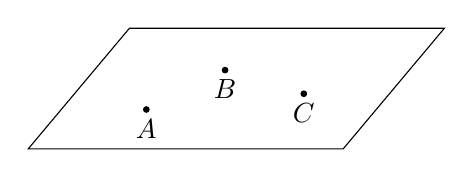
\begin{tikzpicture}[declare function={a=4;}]
		\draw (0,0)--(a,0)--++(50:a/2)--++(-a,0)--cycle;
		\foreach \x/\n in {(1.5,.5)/A, (2.5,1)/B, (3.5,.7)/C}{
			\draw[fill=black] \x circle (1pt) node[below]{$\n$};
		}
		\end{tikzpicture}
	}
\end{tc}
\begin{note}
	Mặt phẳng đi qua ba điểm $A$, $B$, $C$ không thẳng hàng được kí hiệu là mặt phẳng $(ABC)$.
\end{note}

\begin{vd}%[1H4N1-1]%[Dự án đề cương 2025]%[Trịnh Văn Cảnh]
	\immini{
		Cho đường thẳng $a$ đi qua hai điểm phân biệt $M$, $N$ và điểm $O$ không thuộc $a$. Có bao nhiêu mặt phẳng đi qua ba điểm $M$, $N$, $O$?
	}{
		\begin{tikzpicture}[font=\footnotesize]
		\path (0,0) coordinate (M)
		(2,.7) coordinate (N)
		(.8,1.4) coordinate (O);
		\draw[shorten <=-.7 cm, shorten >=-1 cm] (M)--(N);
		\foreach \t/\g in {M/90,N/90,O/90}{
			\draw[fill=black] (\t) circle (1pt) node[shift={(\g:7pt)}]{$\t$};
		}
		\path ($(M)!1.3!(N)$)node[below]{$a$};
		\end{tikzpicture}
	}
	\loigiai{
		
		Do $O$ không thuộc $a$ nên ba điểm $M$, $N$, $O$ không thẳng hàng. Do đó chỉ có một mặt phẳng đi qua ba điểm $M$, $N$, $O$.	
	}
\end{vd}

\begin{tc}
	\immini{
		Nếu một đường thẳng có hai điểm phân biệt thuộc một mặt phẳng thì mọi điểm của đường thẳng đều thuộc mặt phẳng đó.
	}{
		\begin{tikzpicture}[declare function={a=4;}]
		\draw (0,0)coordinate(a)--(a,0)coordinate(b)--++(50:a/2)coordinate(c)--++(-a,0)coordinate(d)--cycle;
		\path (1.5,.5) coordinate (A)
		(3,.7) coordinate (B)
		;
		\foreach \x in {A, B}{
			\draw[fill=black] (\x) circle (1pt) node[below]{$\x$};
		}
		\draw pic[draw, angle radius=6mm]{angle=b--a--d};
		\path (a)+(28:11pt) node{$P$};
		\draw[shorten <=-.7 cm, shorten >=-1 cm] (A)--(B);
		\path ($(A)!1.3!(B)$)node[above]{$d$};
		\end{tikzpicture}
	}
\end{tc}
\begin{note}
	Đường thẳng $d$ nằm trong mặt phẳng $(P)$ thường được kí hiệu là $d \subset (P)$ hoặc $(P) \supset d$.
\end{note}

\begin{vd}%[1H4N1-1]%[Dự án đề cương 2025]%[Trịnh Văn Cảnh]
	Cho ba điểm $A$, $B$, $C$ không thẳng hàng và một điểm $M$ nằm trên đường thẳng $BC$. Gọi $(P)$ là mặt phẳng đi qua ba điểm $A$, $B$, $C$. Chứng tỏ rằng $M \in(P)$.
	\loigiai{
		\immini{
			Áp dụng tính chất 2, ta có $(P)$ là mặt phẳng duy nhất đi qua ba điểm $A, B, C$. Áp dụng tính chất 3, ta có mọi điểm của đường thẳng $BC$ đều thuộc mặt phẳng $(P)$. Ta lại có $M\in BC$ (giả thiết). Suy ra $M \in(P)$.
		}{
			\begin{tikzpicture}[declare function={a=4;}, font=\footnotesize]
			\draw (0,0)coordinate(a)--(a,0)coordinate(b)--++(50:a/2)coordinate(c)--++(-a,0)coordinate(d)--cycle;
			\path (1.5,.7) coordinate (B)
			(3,1) coordinate (C)
			(2.3,.4) coordinate (A)
			($(B)!1.35!(C)$) coordinate (M)
			;
			\foreach \x in {A, B, C, M}{
				\draw[fill=black] (\x) circle (1pt) node[below]{$\x$};
			}
			\draw pic[draw, angle radius=6mm]{angle=b--a--d};
			\path (a)+(28:11pt) node{$P$};
			\draw[shorten >=-1 cm] (B)--(M);
			\draw (C)--(A)--(B);
			\end{tikzpicture}
		}
	}
\end{vd}

\begin{tc}
	Tồn tại bốn điểm không cùng nằm trên một mặt phẳng.
\end{tc}
\begin{note}
	Nếu có nhiều điểm cùng thuộc một mặt phẳng thì ta nói những điểm đó đồng phẳng, còn nếu không có mặt phẳng nào chứa các điểm đó thì ta nói chúng không đồng phẳng.
\end{note}

\begin{vd}%[1H4N1-1]%[Dự án đề cương 2025]%[Trịnh Văn Cảnh]
	Cho bốn điểm $A$, $B$, $C$, $D$ không cùng nằm trên một mặt phẳng. Có bao nhiêu mặt phẳng đi qua ba trong bốn điểm đã cho?
	\loigiai{
		Gọi $A$, $B$, $C$, $D$ là bốn điểm không cùng nằm trên một mặt phẳng trong không gian (tồn tại theo tính chất $4$). Ta xác định được bốn mặt phẳng phân biệt là: $(ABC)$, $(ABD)$, $(ACD)$, $(BCD)$.
	}
\end{vd}

\begin{tc}
	\immini{
		Nếu hai mặt phẳng phân biệt có một điểm chung thì chúng có một đường thẳng chung duy nhất chứa tất cả các điểm chung của hai mặt phẳng đó.
	}{
		\begin{tikzpicture}[declare function={a=2.5;},font=\footnotesize]
		\path 
		(0,0) coordinate (a)
		(0,-a) coordinate (b)
		(b)+(-20:a/1.5) coordinate (c)
		($(a)+(c)-(b)$) coordinate (d)
		(b)+(220:a/1.5) coordinate (e)
		($(a)+(e)-(b)$) coordinate (f)
		($(a)!.35!(b)$) coordinate (M)
		;
		\draw (a)--(b)--(c)--(d)--cycle
		(b)--(e)--(f)--(a)
		;
		\draw pic[draw, angle radius=5mm]{angle=e--f--a};
		\path (f)+(-28:8pt) node{$\alpha$};
		\draw pic[draw, angle radius=5mm]{angle=a--d--c};
		\path (d)+(225:8pt) node{$\beta$};
		\path ($(a)!.7!(b)$)node[right]{$d$};
		\draw[fill=black] (M)node[right]{$M$} circle (1pt);
		\end{tikzpicture}
	}
\end{tc}
\begin{note}
	Đường thẳng $d$ chung của hai mặt phẳng $(P)$ và $(Q)$ được gọi là giao tuyến của $(P)$ và $(Q)$, kí hiệu $d=(P) \cap(Q)$.
\end{note}

\begin{vd}%[1H4N1-3]%[Dự án đề cương 2025]%[Trịnh Văn Cảnh]
	Cho tam giác $ABC$ và một điểm $O$ không thuộc mặt phẳng $(ABC)$. Xác định giao tuyến của hai mặt phẳng $(OAB)$ và $(ABC)$.
	\loigiai{
		Ta có $A$, $B$ là hai điểm chung của hai mặt phẳng $(OAB)$ và $(ABC)$. Suy ra $AB$ là giao tuyến của hai mặt phẳng $(OAB)$ và $(ABC)$.
	}
\end{vd}

\begin{tc}
	Trong mỗi mặt phẳng, các kết quả đã biết của hình học phẳng đều đúng.
\end{tc}

\subsubsection{Cách xác định một mặt phẳng}
\immini{
	\begin{itemize}
		\item Một mặt phẳng được xác định nếu biết nó chứa ba điểm không thẳng hàng.
	\end{itemize}	
	\textit{Mặt phẳng xác định bởi ba điểm $A$, $B$, $C$ không thẳng hàng kí hiệu là mp$(ABC)$ hay $(ABC)$.}
}{
	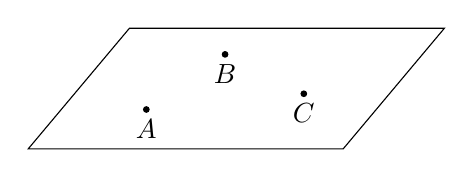
\begin{tikzpicture}[declare function={a=4;}]
	\draw (0,0)--(a,0)--++(50:a/2)--++(-a,0)--cycle;
	\foreach \x/\n in {(1.5,.5)/A, (2.5,1.2)/B, (3.5,.7)/C}{
		\draw[fill=black] \x circle (1pt) node[below]{$\n$};
	}
	\end{tikzpicture}
}
\immini{
	\begin{vd}%[1H4H1-1]%[Dự án đề cương 2025]%[Trịnh Văn Cảnh]
		Cho ba điểm $A$, $B$, $C$ không thẳng hàng và không nằm trong mặt phẳng $(P)$. Biết ba đường thẳng $AB$, $AC$, $BC$ lần lượt cắt $(P)$ tại các điểm $M$, $N$, $E$. Ba điểm $M$, $N$, $E$ có thẳng hàng không? Giải thích.
		\loigiai{
			Gọi $(Q)$ là mặt phẳng xác định bởi ba điểm $A$, $B$, $C$. \\
			Ta có $M \in AB$ và $AB \subset(Q)$, suy ra $M \in(Q)$.\\
			Mặt khác, $M \in(P)$. Vậy $M \in(P) \cap(Q)$.\\
			Tương tự, ta cũng có $N \in(P) \cap(Q)$ và $E \in(P) \cap(Q)$.\\
			Suy ra ba điểm $M$, $N$, $E$ thẳng hàng vì cùng nằm trên đường thẳng giao tuyến của hai mặt phẳng $(P)$ và $(Q)$.
		}
	\end{vd}
}{
	\begin{tikzpicture}[declare function={a=4;}]
	\draw (0,0)coordinate(a)--(a,0)coordinate(b)--++(50:a/2)coordinate(c)--++(-a,0)coordinate(d)--cycle;
	\path (1.5,.5) coordinate (M)
	(3,.7) coordinate (N)
	($(M)!1.75!(N)$) coordinate (E)
	(2,3.5) coordinate (A)
	($(A)!.4!(M)$) coordinate (B)
	(intersection of B--E and A--N) coordinate (C);
	;
	\fill[orange!30] (A)--(B)--(C)--cycle;
	\foreach \t/\g in {A/90,M/-90,N/-90,E/-90,B/180,C/30}{
		\draw[fill=black] (\t) circle (1pt) node[shift={(\g:7pt)}]{$ \t $};
	}
	\draw pic[draw, angle radius=6mm]{angle=b--a--d};
	\path (a)+(28:11pt) node{$P$};
	\draw (A)--(M) (A)--(N) (B)--(E); 
	\end{tikzpicture}
}
\immini{
	\begin{itemize}
		\item Một mặt phẳng được xác định nếu biết nó chứa một đường thẳng và một điểm không thuộc đường thẳng đó.
	\end{itemize}		
	\textit{Mặt phẳng xác định bởi điểm $A$ và đường thẳng $a$ không qua điểm $A$ kí hiệu là mp$(A, a)$ hay $(A, a)$.}
}{
	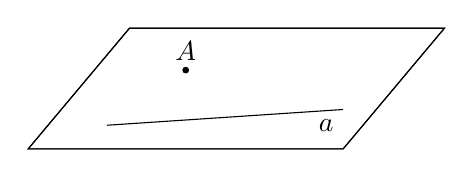
\begin{tikzpicture}[declare function={a=4;}]
	\draw (0,0)coordinate(a)--(a,0)coordinate(b)--++(50:a/2)coordinate(c)--++(-a,0)coordinate(d)--cycle;
	;
	\draw (a)--(b)--(c)--(d)--cycle;
	\draw (1,.3)--(4,.5)node[below left]{$a$};
	\draw[fill=black] (2,1)node[above]{$A$} circle (1pt);
	\end{tikzpicture}
}

\immini{
	\begin{vd}%[1H4N1-1]%[Dự án đề cương 2025]%[Trịnh Văn Cảnh]
		Với đường thẳng $d$ và hai điểm $M$, $N$ phân biệt không thuộc $d$, ta xác định được bao nhiêu mặt phẳng?
		\loigiai{
			Với đường thẳng $d$ và điểm $M$ không thuộc $d$, ta xác định được mặt phẳng thứ nhất là $(M, d)$. Nếu điểm $N$ thuộc $(M, d)$ thì ta chỉ xác định được một mặt phẳng. Nếu điểm $N$ không thuộc $(M, d)$ thì ta xác định được mặt phẳng thứ hai là $(N, d)$.
		}
	\end{vd}
}{
	\begin{tikzpicture}[declare function={a=2.5;},font=\footnotesize]
	\path 
	(0,0) coordinate (a)
	(0,-a) coordinate (b)
	(b)+(-20:a/1.5) coordinate (c)
	($(a)+(c)-(b)$) coordinate (d)
	(b)+(220:a/1.5) coordinate (e)
	($(a)+(e)-(b)$) coordinate (f)
	(-1,-2) coordinate (M)
	(.8,-1.5) coordinate (N)
	;
	\draw (a)--(b)--(c)--(d)--cycle
	(b)--(e)--(f)--(a)
	;
	\path ($(a)!.4!(b)$)node[left]{$d$};
	\foreach \t/\g in {M/90,N/90}{
		\draw[fill=black] (\t) circle (1pt) node[shift={(\g:7pt)}]{$ \t $};
	}
	\end{tikzpicture}
}

\immini{
	\begin{itemize}
		\item Một mặt phẳng được xác định nếu biết nó chứa hai đường thẳng cắt nhau.
	\end{itemize}	
	\textit{Mặt phẳng xác định bởi điểm hai đường thẳng $a$, $b$ cắt nhau kí hiệu là mp$(a, b)$.}
}{
	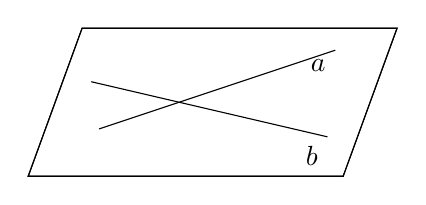
\begin{tikzpicture}[declare function={a=4;}]
	\draw (0,0)coordinate(a)--(a,0)coordinate(b)--++(70:a/2)coordinate(c)--++(-a,0)coordinate(d)--cycle;
	;
	\draw (a)--(b)--(c)--(d)--cycle;
	\draw (.9,.6)--(3.9,1.6)node[below left]{$a$};
	\draw (.8,1.2)--(3.8,.5)node[below left]{$b$};
	\end{tikzpicture}
}

\immini{
	\begin{vd}%[1H4N1-1]%[Dự án đề cương 2025]%[Trịnh Văn Cảnh]
		Với ba đường thẳng $a$, $b$, $c$ không cùng nằm trong một mặt phẳng và cùng đi qua một điểm $O$, ta xác định được bao nhiêu mặt phẳng?
		\loigiai{
			Từ ba cặp đường thẳng cắt nhau $a$ và $b$, $b$ và $c$, $c$ và $a$, ta xác định được ba mặt phẳng là mp$(a, b)$, mp$(b, c)$, mp$(c, a)$.
		}
	\end{vd}
}{
	\begin{tikzpicture}[declare function={a=2.5;},font=\footnotesize]
	\path 
	(0,0) coordinate (O)
	(-130:a) coordinate (A)
	(-80:a) coordinate (B)
	(-30:a) coordinate (C)
	;
	\draw[shorten <=-1cm] (O)--(A)node[left]{$a$};
	\draw[shorten <=-1cm] (O)--(B)node[above right]{$b$};
	\draw[shorten <=-1cm] (O)--(C)node[right]{$c$};
	\foreach \t/\g in {O/0}{
		\draw[fill=black] (\t) circle (1pt) node[shift={(\g:7pt)}]{$ \t $};
	}
	\end{tikzpicture}
}

\textbf{Hình chóp} \\
Cho đa giác lồi $A_1A_2\ldots A_n$ nằm trong mặt phẳng $(\alpha)$ và điểm $S$ không thuộc $(\alpha)$. Nối $S$ với các đỉnh $A_1$, $A_2$, \ldots, $A_n$ ta được $n$ tam giác $SA_1A_2$, $SA_2A_3$, \ldots, $SA_nA_1$. Hình tạo bởi $n$ tam giác đó và đa giác $A_1A_2\ldots A_n$ được gọi là hình chóp, kí hiệu $S.A_1A_2\ldots A_n$.
\immini{
	Trong hình chóp $S.A_1A_2\ldots A_n$, ta gọi:
	\begin{itemize}
		\item Điểm $S$ là \textbf{đỉnh};
		\item Các tam giác $SA_1A_2$, $SA_2A_3$,\ldots, $SA_nA_1$ là các \textbf{mặt bên};
		\item Đa giác $A_1A_2\ldots A_n$ là \textbf{mặt đáy};
		\item Các đoạn thẳng $SA_1$, $SA_2$, \ldots, $SA_n$ là các \textbf{cạnh bên};
		\item Các cạnh của đa giác $A_1A_2\ldots A_n$ là các \textbf{cạnh đáy}.
	\end{itemize}	
	Ta gọi hình chóp có đáy tam giác, tứ giác, ngũ giác,\ldots lần lượt là hình chóp tam giác, hình chóp tứ giác, hình chóp ngũ giác, \ldots
}{
	\begin{tikzpicture}[font=\footnotesize]
	\path 
	(.61,4.37) coordinate (A)
	(-.53,2.12) coordinate (B)
	(0,0) coordinate (C)
	(1.98,0.42) coordinate (D)
	(2.91,1.53) coordinate (E)
	(7.12,4.42) coordinate (F)
	(5.27,1.59) coordinate (G)
	(5.85,.19) coordinate (H)
	(7.3,-.11) coordinate (I)
	(8.81, 1.48) coordinate (J)
	(7.62,2.17) coordinate (K);
	\fill[gray!30] (A)--(D)--(E)--cycle;
	\fill[gray!40] (F)--(G)--(H)--cycle;
	\draw (A)--(B)--(C)--(D)--(E)--cycle (A)--(C) (A)--(D)
	(F)--(G)--(H)--(I)--(J)--cycle (F)--(H) (F)--(I);
	;
	\draw[dashed] (B)--(E) (G)--(K)--(J) (F)--(K);
	\foreach \x/\g/\n in {A/90/S,B/180/A,C/-90/B,D/-90/C,E/0/D,F/90/S,G/180/A,H/225/B,I/-90/C,J/0/D,K/20/E} 
	\draw[fill=black] (\x)circle (1pt)+(\g:7pt)  node {$\n$};
	\node (dinh) at ($(A)!.5!(F)+(0,.3)$){Đỉnh};
	\node (canhben) at ($(A)!.5!(F)+(0,-1)$) {Cạnh bên};
	\node (matben) at ($(A)!.5!(F)+(0,-2)$) {Mặt bên};
	\node (canhday) at ($(A)!.5!(F)+(0,-4)$) {Cạnh đáy};
	\draw 
	(A)--(dinh)--(F)
	($(A)!.4!(E)$)--(canhben)--($(F)!.4!(G)$)
	($(A)!.6!($(D)!.5!(E)$)$)--(matben)--($(F)!.6!($(G)!.5!(H)$)$)
	($(D)!.4!(E)$)--(canhday)--($(G)!.4!(H)$)
	;
	\path 
	($(B)!.5!(D)+(.2,-.2)$) node{Mặt đáy}
	($(H)!.5!(K)+(.5,0)$) node{Mặt đáy};
	\end{tikzpicture}
}
\immini{
	\begin{vd}%[1H4N1-1]%[Dự án đề cương 2025]%[Trịnh Văn Cảnh]
		Cho hình chóp $S.ABCD$ (hình vẽ bên). Gọi tên các mặt bên, mặt đáy, cạnh bên, cạnh đáy của hình chóp $S.ABCD$.
		\loigiai{
			Hình chóp $S.ABCD$ có:
			\begin{itemize}
				\item Các mặt bên: $SAB$, $SBC$, $SCD$, $SDA$;
				\item Mặt đáy $ABCD$;
				\item Các cạnh bên: $SA$, $SB$, $SC$, $SD$;
				\item Các cạnh đáy: $AB$, $BC$, $CD$, $DA$.
			\end{itemize}	
		}
	\end{vd}
}{
	\begin{tikzpicture}[declare function={a=2.5;},font=\footnotesize]
	\path 
	(0,0) coordinate (A)
	(1.8,-1.2) coordinate (B)
	(4.5,-.3) coordinate (C)
	($(A)+(C)-(B)$) coordinate (D)
	(2.5,3) coordinate (S)
	;
	\draw (S)--(A)--(B)--(C)--cycle (S)--(B);
	\draw[dashed] (A)--(D)--(C) (S)--(D);
	\foreach \t/\g in {A/180,B/-90,C/0,D/30,S/90}{
		\draw[fill=black] (\t) circle (1pt) node[shift={(\g:7pt)}]{$ \t $};
	}
	\end{tikzpicture}
}
\noindent\textbf{Hình tứ diện} \\
\immini{
	Cho bốn điểm $A$, $B$, $C$, $D$ không đồng phẳng. Hình tạo bởi bốn tam giác $ABC$, $ACD$, $ADB$ và $BCD$ được gọi là hình tứ diện (hay tứ diện), kí hiệu $ABCD$.\\
	Trong tứ diện $ABCD$, ta gọi:
	\begin{itemize}
		\item Các điểm $A$, $B$, $C$, $D$ là các \textbf{đỉnh}.
		\item Các đoạn thẳng $AB$, $AC$, $AD$, $BC$, $CD$, $BD$ là các \textbf{cạnh} của tứ diện.
		\item Hai cạnh không đi qua một đỉnh là \textbf{hai cạnh đối diện}.
		\item Các tam giác $ABC$, $ACD$, $ADB$, $BCD$ là các \textbf{mặt} của tứ diện.
		\item Đỉnh không thuộc một mặt của tứ diện là \textbf{đỉnh đối diện} với mặt đó.
	\end{itemize}	
}{
	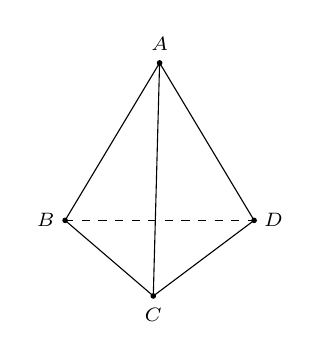
\begin{tikzpicture}[scale=.8,font=\footnotesize]
	\path (0,0) coordinate (B)
	(3,0) coordinate (D)
	(1.4,-1.2) coordinate (C)
	(1.5,2.5) coordinate (A);
	\draw (A)--(B)--(C)--(D)--cycle (A)--(C);
	\draw[dashed] (B)--(D);
	\foreach \t/\g in {A/90,B/180,C/-90,D/0}{
		\draw[fill=black] (\t) circle (1pt) node[shift={(\g:7pt)},font=\scriptsize]{$\t$};
	}
	\end{tikzpicture}
}
\immini{
	\begin{vd}%[1H4N1-1]%[Dự án đề cương 2025]%[Trịnh Văn Cảnh]
		Gọi tên các mặt, các cặp cạnh đối diện của tứ diện $MNPQ$.
		\loigiai{
			Tứ diện $MNPQ$ có:
			\begin{itemize}
				\item Các mặt: $MNP$, $MPQ$, $MQN$, $NPQ$.
				\item Các cặp cạnh đối diện: $MN$ và $PQ$, $MP$ và $NQ$, $MQ$ và $NP$.	
			\end{itemize}	
		}
	\end{vd}
}{
	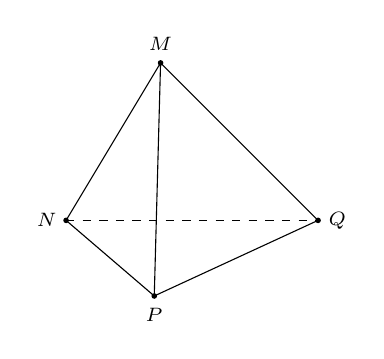
\begin{tikzpicture}[scale=.8,font=\footnotesize]
	\path (0,0) coordinate (N)
	(4,0) coordinate (Q)
	(1.4,-1.2) coordinate (P)
	(1.5,2.5) coordinate (M);
	\draw (M)--(N)--(P)--(Q)--cycle (M)--(P);
	\draw[dashed] (N)--(Q);
	\foreach \t/\g in {M/90,N/180,P/-90,Q/0}{
		\draw[fill=black] (\t) circle (1pt) node[shift={(\g:7pt)},font=\scriptsize]{$\t$};
	}
	\end{tikzpicture}
}
\begin{note}
	\textbf{Chú ý:}
	\begin{itemize}
		\item Hình tứ diện có bốn mặt là các tam giác đều được gọi là hình tứ diện đều.
		\item Một tứ diện có thể xem như là một hình chóp tam giác với đỉnh là một đỉnh tuỳ ý của tứ diện và đáy là mặt của tứ diện không chứa đỉnh đó.
	\end{itemize}	
\end{note}
%-------------------------------------------------------------------------------------------------------------
\subsection{PHÂN LOẠI VÀ PHƯƠNG PHÁP GIẢI TOÁN}
\begin{dang}{Xác định giao tuyến của hai mặt phẳng}
	Để tìm giao tuyến của hai mặt phẳng phân biệt $(P)$, $(Q)$ ta đi tìm hai điểm phân biệt $A$, $B$ thuộc cả hai mặt phẳng đó.
\end{dang}
\begin{vd}%[1H4H1-3]%[Dự án đề cương 2025]%[Trịnh Văn Cảnh]
	Cho $S$ là một điểm không thuộc mặt phẳng hình bình hành $ABCD$. Tìm giao tuyến của hai mặt phẳng $(SAC)$ và $(SBD)$.
	\loigiai
	{
		\immini
		{
			Gọi $O=AC\cap BD$.\\ Ta có $S$ và $O$ là hai điểm chung của $(SAC)$ và $(SBD)$ nên $(SAC)\cap (SBD)=SO$.
		}{
			\begin{tikzpicture}[scale=1,font=\footnotesize,line join=round,line cap=round,>=stealth] 
			\path 
			(0,0) coordinate (A) 
			(-1,-1) coordinate (B) 
			($(A)+(3,0)$) coordinate (D) 
			($(B)+(3,0)$) coordinate (C) 
			($(A)+(0.5,2)$) coordinate (S);
			\path (intersection of A--C and B--D) coordinate (O); 
			\draw[dashed] (C)--(A)--(D)--(B)--(A)--(S)--(O); 
			\draw (S)--(B)--(C)--(D)--(S)--(C); 
			\foreach \p/\g in {S/135,A/135,B/-135,C/-45,D/45,O/-90} 
			\fill[black](\p) circle (1pt) ($(\p)+(\g:3mm)$) node{$\p$}; 
			\end{tikzpicture}}
	}
\end{vd}
\begin{vd}%[1H4H1-3]%[Dự án đề cương 2025]%[Trịnh Văn Cảnh]
	Cho hình chóp $S.ABCD$, đáy là tứ giác $ABCD$ có hai cạnh đối diện $AB$ và $CD$ không song song. Lấy điểm $M$ thuộc miền trong của tam giác $SCD$. Tìm giao tuyến của hai mặt phẳng:
	\begin{listEX}[3]
		\item $(SBM)$ và $(SCD)$;
		\item $(ABM)$ và $(SCD)$;
		\item $(ABM)$ và $(SAC)$.
	\end{listEX}
	\loigiai
	{
		\begin{center}
			\begin{tikzpicture}[scale=1,font=\footnotesize,line join=round,line cap=round,>=stealth] 
			\path 
			(0,0) coordinate (A) 
			(1,-1.5) coordinate (B) 
			(3,-2) coordinate (C) 
			(5,0.5) coordinate (D) 
			(2,3) coordinate (S)
			(3,1) coordinate (M)
			($(S)!1.92!(M)$) coordinate (E)
			(intersection of A--B and C--D) coordinate (I)
			(intersection of I--M and S--C) coordinate (J); 
			\draw[-] (M)--(E);
			\draw[dashed] (B)--(C) (A)--(D) (A)--(M)--(B) (A)--(J); 
			\draw (S)--(A)--(B)--cycle (S)--(C)--(D)--cycle (B)--(I)--(C) (S)--(M)--(I); 
			\foreach \p/\g in {S/135,A/135,B/-135,C/-45,D/45,M/45,I/-90,J/-135} 
			\fill[black](\p) circle (1pt) ($(\p)+(\g:3mm)$) node{$\p$}; 
			\end{tikzpicture}
		\end{center}
		\begin{enumerate}
			\item $(SBM)\cap (SCD)=?$\\
			Dễ thấy $S$, $M$ là hai điểm chung của hai mặt phẳng $(SBM)$ và $(SCD)$ nên $(SBM)\cap (SCD)=SM$.
			\item $(ABM)\cap (SCD)=?$\\
			Ta thấy $M\in (ABM)\cap (SCD)$.\\
			Gọi $I=AB\cap CD$. Khi đó $I\in AB$ nên $I\in (ABM)$.\\ Mặt khác $I\in CD$ nên $I\in (SCD)$.\\
			Khi đó $(ABM)\cap (SCD)=IM$.
			\item $(ABM)\cap (SAC)=?$\\
			Ta thấy $A\in (ABM)\cap (SAC)$.\\
			Gọi $J=IM\cap SC$. Khi đó $J\in IM$ mà $IM\cap (ABM)$ nên $J\in (ABM)$.\\ Mặt khác $J\in AC $ nên $J\in (SAC)$.\\
			Vậy $(ABM)\cap (SAC)=AJ$.
		\end{enumerate}
	}
\end{vd}
\begin{vd}%[1H4H1-3]%[Dự án đề cương 2025]%[Trịnh Văn Cảnh]
	Cho hình chóp $S.ABCD$ đáy là hình bình hành tâm $O$. Gọi $M$, $N$, $P$ lần lượt là trung điểm của cạnh $BC$, $CD$, $SA$. Tìm giao tuyến của 
	\begin{enumEX}[a)]{2}
		\item $(MNP)$ và $(SAB)$.
		\item $(MNP)$ và $(SBC)$.
	\end{enumEX}
	\loigiai
	{
		\immini
		{
			\begin{enumerate}[a)]
				\item Tìm $(MNP)\cap (SAB)$.
				\begin{itemize}
					\item Ta có $P\in (MNP)\cap (SAB). \qquad (1)$
					\item Gọi $F=MN \cap AB $ thì $\heva{& F\in MN\subset (MNP) \\ & F\in AB\subset (SAB).}$\\
					nên $F\in (MNP)\cap (SAB).\qquad (2)$
				\end{itemize}
				Từ $(1)$ và $(2)$ suy ra $(MNP)\cap (SAB)=PF$.
				\item Tìm $(MNP)\cap (SBC)$.
				\begin{itemize}
					\item Ta có $M\in (MNP)\cap (SBC). \qquad (3)$.
					\item Gọi $K=PF \cap SB $ thì $\heva{& K\in PF\subset (MNP) \\ & K\in SB\subset (SBC).}$\\
					nên $K\in (MNP)\cap (SBC).\qquad (4)$
				\end{itemize}
				Từ $(3)$ và $(4)$ suy ra $(MNP)\cap (SBC)=MK$.
			\end{enumerate}
		}{
			\begin{tikzpicture}[scale=1,font=\footnotesize,line join=round,line cap=round,>=stealth] 
			\path 
			(0,0) coordinate (A) 
			(-1,-1.5) coordinate (D) 
			($(A)+(3,0)$) coordinate (B) 
			($(D)+(3,0)$) coordinate (C) 
			($(A)+(0.5,2)$) coordinate (S)
			($(B)!0.5!(C)$) coordinate (M)
			($(C)!0.5!(D)$) coordinate (N)
			($(S)!0.5!(A)$) coordinate (P)
			(intersection of M--N and A--B) coordinate (F)
			(intersection of S--B and P--F) coordinate (K);
			\draw (S)--(K)--(M)--(C)--(S)--(D)--(C) (K)--(F)--(M); 
			\draw[dashed] (S)--(A)--(F) (A)--(D) (M)--(N)--(P)--(K)--(B)--(M)--(P); 
			\foreach \p/\g in {S/135,A/-60,B/-45,C/-45,D/-135,M/-45,N/-90,P/45,F/45,K/60} 
			\fill[black](\p) circle (1pt) ($(\p)+(\g:3mm)$) node{$\p$}; 
			\end{tikzpicture}}
	}
\end{vd}
\begin{dang}{Tìm giao điểm của đường thẳng và mặt phẳng}
	Muốn tìm giao điểm của một đường thẳng $a$ và mặt phẳng $(P)$, ta tìm giao điểm của $a$ và một đường thẳng $b$ nằm trong $(P)$.\\
	\immini{ $a\cap b=M$ và $b\subset (P)$.\\
		Suy ra $M=a\cap (P)$.
	}
	{\begin{tikzpicture}[line cap=round,line join=round]
		\tkzInit[xmin=-4,xmax=8,ymin=-1,ymax=8]
		\tkzDefPoints{0/0/A, 3/0/B,2/2.5/C, 0.6/3/S}
		\tkzDefPointBy[translation = from A to B](C)
		\tkzGetPoint{D}
		\tkzDefMidPoint(A,C)\tkzGetPoint{I}
		\tkzDefMidPoint(B,D)\tkzGetPoint{K}
		\tkzDefPointBy[translation = from I to S](K)
		\tkzGetPoint{Q}
		\tkzDefPointBy[homothety=center S ratio 1/4](K)\tkzGetPoint{Z}
		\tkzDefPointBy[homothety=center I ratio 2/3](K)\tkzGetPoint{M}
		\tkzInterLL(Q,K)(C,D)\tkzGetPoint{Y}
		\tkzDrawPoints[fill=black](M)
		\tkzLabelSegments[ below left](I,K){$b$}
		\tkzLabelSegments[ right](M,Z){$a$}
		\tkzLabelPoint[ below](M){$M$}
		\tkzLabelPoint[above right](A){$\quad P$}
		\tkzLabelPoint[below right](S){$Q$}
		\tkzDrawSegments(A,B A,I B,D I,K Y,D S,I S,Q Q,K M,Z) 
		\tkzDrawSegments[dashed](I,C C,Y)
		\end{tikzpicture}
	}
	%
	\textbf{Phương pháp:}\\
	\textbf{- Bước 1:} Xác định mặt phẳng $(Q)$ chứa $a$.\\
	\textbf{- Bước 2:} Tìm giao tuyến $b=(P) \cap (Q)$.\\
	\textbf{- Bước 3:} Gọi $M=a\cap b$. Suy ra $M= a\cap (P)$.
	
\end{dang}
%
\begin{vd}%[1H4H1-4]%[Dự án đề cương 2025]%[Trịnh Văn Cảnh]
	Cho tứ diện $ABCD$. Gọi $I$ là điểm trên cạnh $AB$ sao cho $AI=\dfrac{1}{3}AB$ và $G$ là trọng tâm của tam giác $ACD$. Tìm giao điểm của đường thẳng $IG$ với mặt phẳng $BCD$.
	\loigiai
	{
		\immini
		{
			\begin{itemize}
				\item Gọi $M$ là trung điểm của $CD$.
				\item Trong mặt phẳng $ABM$, gọi $E=IG\cap BM$.
				\item Khi đó $\heva{&E\in IG\\&E\in BM\subset (BCD)}\Rightarrow IG\cap (BCD)=E$.
			\end{itemize}
		}{
			\begin{tikzpicture}[scale=1,font=\footnotesize,line join=round,line cap=round,>=stealth] 
			\path 
			(0,0) coordinate (B) 
			(1.5,-1.5) coordinate (C) 
			(5,0) coordinate (D) 
			(2,3) coordinate (A)
			($(A)!1/3!(B)$) coordinate (I)
			($(C)!0.5!(D)$) coordinate (M)
			($(A)!2/3!(M)$) coordinate (G)
			($(M)!0.4!(D)$) coordinate (K)
			(intersection of I--G and B--M) coordinate (E); 
			\draw (A)--(B)--(C)--(A)--(D)--(K) (A)--(M)--(E)--(G) (M)--(C); 
			\draw[dashed] (K)--(M)--(B)--(D) (I)--(G) ; 
			\foreach \p/\g in {A/90,B/180,C/-90,D/-45,I/135,G/30,M/-90,E/30} 
			\fill[black](\p) circle (1pt) ($(\p)+(\g:3mm)$) node{$\p$};
			\path 
			(C)--(M) node[pos=0.5,sloped,scale=0.5]{$//$}
			(D)--(M) node[pos=0.5,sloped,scale=0.5]{$//$}; 
			\end{tikzpicture}}
	}
\end{vd}
\begin{vd}%[1H4H1-4]%[Dự án đề cương 2025]%[Trịnh Văn Cảnh] 
	Cho tứ diện $ABCD$. Trên cạnh $AC$, $AD$ lần lượt lấy hai điểm $M$ và $N$ sao cho $AC=3AM$, $3AN=2AD$. Gọi $O$ là điểm thuộc miền trong của tam giác $BCD$. Tìm giao điểm của $BD$ và mặt phẳng $(OMN)$.
	\loigiai
	{
		\immini
		{
			\begin{itemize}
				\item Trong mặt phẳng $(ACD)$, gọi $I=MN\cap CD$.
				\item Khi đó $\heva{&I\in CD\subset (BCD)\Rightarrow OI\subset (BCD)\\&I\in MN\subset (OMN)\Rightarrow OI\subset (OMN).}$
				\item Trong mặt phẳng $(BCD)$, gọi $J=BD\cap OI$.
				\item Khi đó $\heva{&J\in BD\\&J\in OI\subset (OMN)}\Rightarrow BD\cap (OMN)=J$.
			\end{itemize}	
		}{
			\begin{tikzpicture}[scale=1,font=\footnotesize,line join=round,line cap=round,>=stealth] 
			\path 
			(0,0) coordinate (B) 
			(1,-2) coordinate (C) 
			(5,0) coordinate (D) 
			(1.5,3) coordinate (A)
			($(A)!1/3!(C)$) coordinate (M)
			($(A)!2/3!(D)$) coordinate (N)
			($(B)!1.67!(O)$) coordinate (E)
			(2,-0.5) coordinate (O)
			(intersection of M--N and C--D) coordinate (I)
			(intersection of O--I and B--D) coordinate (J); 
			\draw (A)--(B)--(C)--(D)--(A)--(C) (M)--(I)--(D); 
			\draw[dashed] (O)--(B)--(D) (M)--(O)--(N) (E)--(O)--(I); 
			\foreach \p/\g in {A/135,B/-135,C/-135,D/-45,M/180,N/45,O/-90,I/90,J/90} 
			\fill[black](\p) circle (1pt) ($(\p)+(\g:3mm)$) node{$\p$}; 
			\end{tikzpicture}}
	}
\end{vd}
\begin{vd}%[1H4H1-4]%[Dự án đề cương 2025]%[Trịnh Văn Cảnh]
	Cho hình chóp $S.ABCD$ có đáy là hình bình hành. Gọi $M$, $N$ lần lượt là trung điểm của các cạnh $SA$, $BC$. Xác định giao điểm của mặt phẳng $(DMN)$ với các đường thẳng $AB$, $SB$.
	\loigiai{
		\begin{center}
			\begin{tikzpicture}[scale=1, font=\footnotesize, line join=round, line cap=round, >=stealth]
			\def\bc{4} % cạnh BC
			\def\ba{2} % cạnh BA
			\def\h{4} % đường cao
			\def\gocB{35} % góc B của đáy
			\coordinate[label=below left:$D$] (D) at (0,0);
			\coordinate[label=above left:$A$] (A) at (\gocB:\ba);
			\coordinate[label=below:$C$] (C) at (\bc,0);
			\coordinate[label=above right:$B$] (B) at ($(C)-(D)+(A)$);
			\coordinate [label=above:$S$](S) at (70:5);
			\coordinate[label=left:$M$] (M) at ($(S)!1/2!(A)$);
			\coordinate[label=below right:$N$] (N) at ($(B)!1/2!(C)$);
			\path 
			(intersection of A--B and N--D) coordinate (P);
			\node at (P) [right]{$P$};
			\path 
			(intersection of S--B and M--P) coordinate (E);
			\node at (E) [above]{$E$};
			\draw (S)--(D)--(C)--(N)--(E)--cycle (S)--(C) (E)--(P)--(N);
			\draw[dashed] (D)--(A)--(P) (D)--(M)--(N)--cycle (M)--(E)--(B)--(N) (S)--(A);
			\foreach \i in {A,B,C,D,M,N,E,P,S} \fill[black] (\i) circle (1pt);
			\end{tikzpicture}
		\end{center}
		Trong mặt phẳng $(ABCD)$ có $DN$ cắt $AB$ tại $P$. Vì $P \in D N$ nên $P \in(DMN)$.\\ Do đó, $P$ là giao điểm của mặt phẳng $(DMN)$ với $AB$.\\
		Trong mặt phẳng $(SAB)$ có $MP$ cắt $S B$ tại $E$. Vì $E \in MP$ nên $E \in(DMN)$.\\ Do đó, $E$ là giao điểm của mặt phẳng ($DMN)$ với $SB$.
	}	
\end{vd}
\begin{dang}{Chứng minh 3 điểm thẳng hàng và 3 đường thẳng đồng quy}
	\begin{itemize}
		\item {\bf Chứng minh ba điểm thẳng hàng:} Ta chứng minh ba điểm đó cùng thuộc 2 mặt phẳng phân biệt. Khi đó chúng phải cùng thuộc đường thẳng giao tuyến của hai mặt, tức là thẳng hàng.
		\item {\bf Chứng minh ba đường đồng quy:} Giả sử cần chứng minh $AB$, $CD$, $MN$ đồng quy. Ta tìm $K$ là giao điểm của $AB$ và $CD$, sau đó chứng minh $K$, $M$, $N$ thẳng hàng.
	\end{itemize}
\end{dang}
\begin{vd}%[1H4H1-6]%[Dự án đề cương 2025]%[Trịnh Văn Cảnh]
	Cho ba điểm $A$, $B$, $C$ không thuộc mặt phẳng $(Q)$ và các đường thẳng $BC$, $CA$, $AB$ cắt $(Q)$ lần lượt tại $M$, $N$, $P$. Chứng minh rằng $M$, $N$, $P$ thẳng hàng.
	\loigiai{
		\immini{
			Ta có $M=BC \cap (Q)$ nên $M \in BC \subset (ABC)$ và $M \in (Q)$.\\
			$N=AC \cap (Q)$ nên $N \in AC \subset (ABC)$, $N \in (Q)$ \\
			$P=AB \cap (Q)$ nên $P \in AB \subset (ABC)$, $P \in (Q)$.\\
			Do đó $M$, $N$, $P$ nằm trên giao tuyến của hai mặt phẳng $(ABC)$ và $ (Q)$.\\
			Vậy $M$, $N$, $P$ thẳng hàng.
		}{
			\begin{tikzpicture}[scale=1, font=\footnotesize, line join=round, line cap=round, >=stealth]
			\path 
			(0,0) coordinate (a)
			--($(a)+(0:4)$) coordinate (b)
			--($(a)+(50:2)$) coordinate (d)
			--($(b)+(d)-(a)$) coordinate (c)
			(1.3,0.8) coordinate (P)
			--($(P)+(0:1)$) coordinate (N)
			--($(P)!1.8!(N)$) coordinate (M)
			--($(P)+(65:2.5)$) coordinate (A)
			--($(P)!2/3!(A)$) coordinate (B)
			--(intersection of A--N and B--M) coordinate(C);
			;
			\draw (a)--(b)--(c)--(d)--cycle (A)--(P)--(M);
			\begin{scope}
			\clip (a)--(P)--(M)--(b)--cycle;
			\draw[dashed,shorten <= 0cm,shorten >= -0.5cm] (A)--(P);
			\draw[dashed,shorten <= 0cm,shorten >= -0.5cm] (B)--(M);
			\draw[dashed,shorten <= 0cm,shorten >= -0.5cm] (A)--(N);
			\end{scope}
			\begin{scope}
			\clip (B)--(P)--(M)--cycle;
			\fill[white] (B)--(P)--(M)--cycle;
			\draw[dashed] (d)--(c);
			\end{scope}
			\begin{scope}
			\clip (d)--(a)--(b);
			\draw (a) circle (8mm);
			\end{scope}
			\node at ($(a)+(20:15pt)$){$Q$};
			\draw (A)--(N) (B)--(M);
			\foreach \p/\g in {P/-150,N/-150,M/-90,A/0,B/180,C/0}\draw[fill=black] (\p) circle (.7pt)node[shift={(\g:.2)},scale=.8]{$\p$};
			\end{tikzpicture}
		}
	}
\end{vd}
\begin{vd}%[1H4H1-6]%[Dự án đề cương 2025]%[Trịnh Văn Cảnh] 
	Cho hình chóp $S.ABCD$ có $AC$ cắt $BD$ tại $O$ và $AB$ cắt $CD$ tại $P$. Điểm $M$ thuộc cạnh $SA$ ($M$ khác $S$, $M$ khác $A$). Gọi $N$ là giao điểm của $MP$ và $SB$, $I$ là giao điểm của $MC$ và $DN$. Chứng minh rằng $S$, $O$, $I$ thẳng hàng.
	\loigiai{
		\immini{
			Ta có $ \heva{&S\in (SAC)\cap (SDB)\\&O\in (SAC)\cap (SDB)} $ suy ra $ SO= (SAC)\cap (SDB) $.\\
			Xét $ (MPD) $, $ I\in MC\cap DN \Rightarrow \heva{&I\in MC,\,MC\subset (SAC)\\&I\in DN,\,DN\subset (SBD)} $\\ suy ra $I\in (SAC)\cap (SDB) $ hay $ I\in SO $.\\
			Vậy $S$, $O$, $I$ thẳng hàng.
		}
		{
			\begin{tikzpicture}[scale=1, font=\footnotesize, line join=round, line cap=round, >=stealth]
			\def\bc{4} % cạnh BC
			\def\ba{2} % cạnh BA
			\def\h{4} % đường cao
			\def\gocB{135} % góc B của đáy
			\coordinate[label=below left:$B$] (B) at (0,0);
			\coordinate[label=left:$A$] (A) at (\gocB:\ba);
			\coordinate[label=below right:$C$] (C) at ($(B)+(2,-.5)$);
			\coordinate[label=right:$D$] (D) at ($(A)+(5,0)$);
			\coordinate [label=above:$S$](S) at (70:5);
			\coordinate[label=left:$M$] (M) at ($(S)!1/3!(A)$);
			\path 
			(intersection of A--C and B--D) coordinate (O);
			\node at (O) [below]{$O$};
			\path 
			(intersection of A--B and C--D) coordinate (P);
			\node at (P) [below]{$P$};
			\path 
			(intersection of M--P and S--B) coordinate (N);
			\node at (N) [left]{$N$};
			\path 
			(intersection of D--N and C--M) coordinate (I);
			\node at (I) [above right]{$I$};
			\draw (S)--(A)--(P)--(D)--cycle (S)--(P)--(M) (B)--(S)--(C);
			\draw[dashed] (A)--(C)--(B) (A)--(D)--(B) (M)--(C) (D)--(N);
			\draw[dashed, red] (S)--(O);
			\foreach \i in {A,B,C,D,M,N,I,P,S,O} \fill[black] (\i) circle (1pt);
			\end{tikzpicture}
		}
	}	
\end{vd}
\begin{vd}%[1H4V1-6]%[Dự án đề cương 2025]%[Trịnh Văn Cảnh]
	Cho hình chóp tứ giác $S.ABCD$ có đáy không là hình thang. Gọi $O$ là giao điểm của $AC$ và $BD$. Trên $SO$ lấy điểm $I$ sao cho $SI=2IO$.
	\begin{enumEX}{1}
		\item Xác định các giao điểm $M$, $N$ lần lượt của $SA$, $SD$ với mặt phẳng $(IBC)$.
		\item Chứng minh rằng các đường thẳng $AD$, $BC$ và $MN$ đồng quy.
	\end{enumEX}
	\loigiai{\begin{center}
			\begin{tikzpicture}[scale=0.9,font=\footnotesize,line join=round,line cap=round,>=stealth] 
			\path 
			(0,0) coordinate (A) 
			(2,-2) coordinate (B) 
			(4,-1.5) coordinate (C) 
			(6,0) coordinate (D) 
			(3,4) coordinate (S) 
			(intersection of A--C and B--D) coordinate (O)
			($(S)!2/3!(O)$) coordinate (I)
			(intersection of C--I and S--A) coordinate (M)
			(intersection of B--I and S--D) coordinate (N)
			(intersection of A--D and B--C) coordinate (K)
			;
			\draw (A)--(S)--(B)--(C)--(S)--(K)--(B)--(A) ; 
			\draw[dashed] (S)--(N)--(M)--(I)--(C)--(D)--(N)--(K)--(D)(C)--(A)--(D)--(B) --(N) (S)--(O)
			; 
			\foreach \p/\g in {S/135,A/120,B/170,C/-45,D/30,M/125,N/80,K/60,I/170,O/120} 
			\fill[black](\p) circle (1pt) ($(\p)+(\g:3mm)$) node{$\p$}; 	
			\end{tikzpicture}
		\end{center}
				\begin{enumEX}{1}
				\item Trong mặt phẳng $(SAC)$, gọi $M$ là giao điểm của $CI$ và $SA$. Vì $M \in CI$ nên $M \in(IBC)$. Vậy $M$ là giao điểm của $SA$ với mặt phẳng $(IBC)$. Tương tự, trong mặt phẳng $(SBD)$, gọi $N$ là giao điểm của $BI$ với $SD$, khi đó, $N$ là giao điểm của $SD$ với mặt phẳng $(IBC)$.
				\item Do $ABCD$ không là hình thang nên $AD$ cắt $BC$ tại $K$. Ta có $K \in BC \subset(IBC)$, $K \in AD \subset(SAD)$ nên $K$ là một điểm chung của $(IBC)$ và $(SAD)$.\\
				Mà $MN=(IBC) \cap(SAD)$ nên $K \in MN$. Vậy các đường thẳng $AD$, $BC$ và $MN$ cùng đi qua điểm $K$.
		\end{enumEX}}

\end{vd}
%-----------------------------------------------------------------------------
\subsection{Bài tập rèn luyện}
\ind{PHẦN I.} \inden{Câu trắc nghiệm nhiều phương án lựa chọn. Mỗi câu hỏi học sinh chỉ chọn một phương án.}\\
\setcounter{ex}{0}
\Opensolutionfile{ans}[ans/2D1-Bai1-TN]%--Đặt tên 2D1-Bai1-Dang1-TN

\begin{ex}%[1H4N1-1]%[Dự án đề cương 2025]%[Trịnh Văn Cảnh] 
	Trong không gian, mệnh đề nào sau đây đúng?
	\choice{Bốn điểm nào cũng không đồng phẳng}
	{Có nhiều nhất ba điểm không đồng phẳng}
	{\True Có ít nhất bốn điểm không đồng phẳng}
	{Ba điểm nào cũng không đồng phẳng}
	\loigiai{
		Mệnh đề đúng là \lq\lq Có ít nhất bốn điểm không đồng phẳng\rq\rq.
	}
\end{ex}
\begin{ex}%[1H4N1-3]%[Dự án đề cương 2025]%[Trịnh Văn Cảnh]
	Cho tứ diện $ABCD$. Giao tuyến của hai mặt phẳng $(ABC)$ và $(BCD)$ là
	\choice
	{\True $BC$}
	{$AB$}
	{$CD$}
	{$AD$}
	\loigiai{
		$(ABC)\cap (BCD)=BC$.
	}
\end{ex}
\begin{ex}%[1H4N1-3]%[Dự án đề cương 2025]%[Trịnh Văn Cảnh]
	Cho hình chóp $S.ABC$. Gọi $M$ là trung điểm của cạnh $BC$. Giao tuyến của hai mặt phẳng $(SAM)$ và $(SBC)$ là
	\choice
	{$SB$}
	{\True $SM$}
	{$SC$}
	{$BC$}
	\loigiai{\immini{Dễ thấy $(SAM)\cap (SBC)=SM$.}{
			\begin{tikzpicture}[scale=1,font=\footnotesize,line join=round,line cap=round,>=stealth] 
			\path 
			(0,0) coordinate (A) 
			(2,-1) coordinate (B) 
			(3,0) coordinate (C) 
			(1,2) coordinate (S)
			($(B)!0.5!(C)$) coordinate (M); 
			\draw (S)--(A)--(B)--(C)--(S)--(B) (S)--(M); 
			\draw[dashed] (C)--(A)--(M); 
			\foreach \p/\g in {S/135,A/-135,B/-135,C/-45,M/0} 
			\fill[black](\p) circle (1pt) ($(\p)+(\g:3mm)$) node{$\p$}; 
			\end{tikzpicture}}
	}
\end{ex}
\begin{ex}%[1H2H1-1]%[Dự án đề cương 2025]%[Trịnh Văn Cảnh]
	Cho năm điểm phân biệt trong đó không có bốn điểm nào đồng phẳng. Có bao nhiêu mặt phẳng đi qua ba trong năm điểm trên?
	\choice{\True $10 $}
	{$12$}
	{$14$}
	{$8$}
	\loigiai{
		Cứ $3$ điểm không thẳng hàng xác định duy nhất một mặt phẳng, do không có bốn điểm nào đồng phẳng nên số mặt phẳng thỏa mãn bằng $\mathrm{C}^3_5=10$ mặt phẳng.
	}
\end{ex}	

\begin{ex}%[1H4H1-3]%[Dự án đề cương 2025]%[Trịnh Văn Cảnh]
	Cho hình chóp $S.ABCD$, có đáy $ABCD$ là hình bình hành tâm $O$. Khi đó giao tuyến của hai mặt phẳng $(SBO)$ và $(SCD)$ là
	\choice
	{$SA$}
	{$S0$}
	{$SB$}
	{\True $SD$}
	\loigiai
	{
		\immini
		{
			Dễ thấy $S\in (SBO)\cap (SCD)$.\\
			và $D\in (SBO)\cap (SCD)$ nên $(SBO)\cap (SCD)=SD$.
		}{
			\begin{tikzpicture}[scale=1,font=\footnotesize,line join=round,line cap=round,>=stealth] 
			\path 
			(0,0) coordinate (A) 
			(-1,-1) coordinate (B) 
			($(A)+(3,0)$) coordinate (D) 
			($(B)+(3,0)$) coordinate (C) 
			($(A)+(0.5,2)$) coordinate (S)
			(intersection of A--C and B--D) coordinate (O); 
			\draw[dashed] (S)--(A)--(B) (C)--(A)--(D) (B)--(D) (S)--(O); 
			\draw (S)--(B)--(C)--(D)--(S)--(C); 
			\foreach \p/\g in {S/135,A/135,B/-135,C/-45,D/45,O/-90} 
			\fill[black](\p) circle (1pt) ($(\p)+(\g:3mm)$) node{$\p$}; 
			\end{tikzpicture}}
	}
\end{ex}

\begin{ex}%[1H4H1-3]%[Dự án đề cương 2025]%[Trịnh Văn Cảnh]
	Cho hình chóp $S.ABCD$ có đáy $ABCD$ là hình bình hành. Gọi $M$, $N$ lần lượt là trung điểm của $AD$ và $BC$. Giao tuyến của hai mặt phẳng $(SMN)$ và $(SAC)$ là
	\choice
	{$SD$}
	{\True $SO$ ($O$ là tâm của hình bình bình hành $ABCD$)}
	{$SE$ ($E$ là trung điểm của $AB$)}
	{$SF$ ($F$ là trung điểm của $CD$)}
	\loigiai
	{
		\immini
		{
			Dễ thấy $S\in (SMN)\cap (SAC)$.\\
			Gọi $O$ là tâm của hình bình hành $ABCD$ khi đó $O=AC\cap MN$.\\
			$\Rightarrow \heva{&O\in MN\subset (SMN)\\&O\in AC\subset (SAC)}\Rightarrow O\in (SMN)\cap (SAC)$.\\
			Vậy $(SMN)\cap (SAC)=SO$ với $O$ là tâm của hình bình hành $ABCD$.
		}{
			\begin{tikzpicture}[scale=1,font=\footnotesize,line join=round,line cap=round,>=stealth] 
			\path 
			(0,0) coordinate (A) 
			(-1,-1) coordinate (B) 
			($(A)+(4,0)$) coordinate (D) 
			($(B)+(4,0)$) coordinate (C) 
			($(A)+(0.5,3)$) coordinate (S)
			($(A)!0.5!(D)$) coordinate (M)
			($(B)!0.5!(C)$) coordinate (N)
			(intersection of A--C and B--D) coordinate (O); 
			\draw[dashed] (S)--(A)--(B) (C)--(A)--(D) (B)--(D) (S)--(O) (N)--(M)--(S); 
			\draw (N)--(S)--(B)--(C)--(D)--(S)--(C); 
			\foreach \p/\g in {S/135,A/135,B/-135,C/-45,D/45,O/-45,M/-45,N/-90} 
			\fill[black](\p) circle (1pt) ($(\p)+(\g:3mm)$) node{$\p$}; 
			\end{tikzpicture}}	
	}
\end{ex}

\begin{ex}%[1H4H1-3]%[Dự án đề cương 2025]%[Trịnh Văn Cảnh]
	Cho tứ diện $ABCD$, gọi $G_1$, $G_2$ lần lượt là trọng tâm của các tam giác $ACD$ và $BCD$. Giao tuyến của mặt phẳng $(BG_1G_2)$ và mặt phẳng $(ACD)$ là 
	\choice
	{$G_1G_2$}
	{\True $AG_1$}
	{$AG_2$}
	{$CG_1$}
	\loigiai{\immini{Dễ thấy $G_1\in (BG_1G_2)\cap (ACD).\qquad (1)$\\
			Gọi $M$ là trung điểm $CD$, khi đó $M\in BG_2$ hay $M\in (BG_1G_2)$.\\
			Từ đó suy ra $MG_1\subset (BG_1G_2)$ mà $A\in (MG_1)\Rightarrow A\in (BG_1G_2)$.\\
			Do đó $A\in (ACD)\cap (BG_1G_2).\qquad (2)$\\
			Vậy $AG_1$ là giao tuyến của hai mặt phẳng $(BG_1G_2)$ và $(ACD)$.}{
			\begin{tikzpicture}[scale=1,font=\footnotesize,line join=round,line cap=round,>=stealth] 
			\path 
			(0,0) coordinate (B) 
			(1.5,-1.5) coordinate (C) 
			(5,0) coordinate (D) 
			(2,3) coordinate (A)
			($(C)!0.5!(D)$) coordinate (M)
			($(A)!2/3!(M)$) coordinate (G_1)
			($(B)!2/3!(M)$) coordinate (G_2); 
			\draw (M)--(A)--(B)--(C)--(D)--(A)--(C); 
			\draw[dashed] (B)--(D) (M)--(B)--(G_1)--(G_2); 
			\foreach \p/\g in {A/90,B/180,C/-90,D/-45,M/-30,G_1/45,G_2/-90} 
			\fill[black](\p) circle (1pt) ($(\p)+(\g:3mm)$) node{$\p$};
			\path 
			(C)--(M) node[pos=0.5,sloped,scale=0.5]{$//$}
			(D)--(M) node[pos=0.5,sloped,scale=0.5]{$//$}; 
			\end{tikzpicture}}
	}
\end{ex}

\begin{ex}%[1H4H1-3]%[Dự án đề cương 2025]%[Trịnh Văn Cảnh]
	Cho hình chóp tứ giác $S.ABCD$ và $M$ là điểm bất kỳ trên cạnh $SD$. Giao tuyến của hai mặt phẳng $(SBD)$ và $(MAC)$ là
	\choice
	{$SO$ với $O$ là giao điểm của $AC$ và $BD$}
	{$OM$ với $O$ là giao điểm của $MC$ và $BD$}
	{\True $OM$ với $O$ là giao điểm của $AC$ và $BD$}
	{$OM$ với $O$ là giao điểm của $SB$ và $AC$}
	\loigiai
	{
		\immini
		{Ta có $\heva{&M\in SD \Rightarrow M\in (SBD)\\&M\in (MAC)}\Rightarrow M\in (SBD)\cap (MAC).\qquad (1)$\\
			Gọi $O\in AC\cap BD$.\\
			Khi đó $\heva{&O\in BD \Rightarrow O\in (SBD)\\&O\in AC\Rightarrow O\in (MAC)}\Rightarrow  O\in (SBD)\cap (MAC).\qquad (2)$\\
			Từ $(1)$ và $(2)$ suy ra $OM$ là giao tuyến của hai mặt phẳng $(SBD)$ và $(MAC)$.
		}{
			\begin{tikzpicture}[scale=1,font=\footnotesize,line join=round,line cap=round,>=stealth] 
			\path 
			(0,0) coordinate (A) 
			(1,-1) coordinate (B) 
			(3,-1.5) coordinate (C) 
			(5,0) coordinate (D) 
			(2,3) coordinate (S)
			($(S)!0.6!(D)$) coordinate (M)
			(intersection of A--C and B--D) coordinate (O);
			\draw[dashed] (M)--(A)--(D)--(B) (A)--(C) (M)--(O); 
			\draw (B)--(S)--(A)--(B)--(C)--(D)--(S)--(C)--(M); 
			\foreach \p/\g in {S/135,A/135,B/-135,C/-45,D/45,M/30,O/90} 
			\fill[black](\p) circle (1pt) ($(\p)+(\g:3mm)$) node{$\p$}; 
			\end{tikzpicture}}
	}
\end{ex}

\begin{ex}%[1H4H1-3]%[Dự án đề cương 2025]%[Trịnh Văn Cảnh]
	Cho hình chóp $S.ABCD$ có đáy là hình thang $(AB\parallel CD)$. Khẳng định nào sau đây \textbf{sai}?
	\choice
	{Hình chóp $S.ABCD$ có bốn mặt bên}
	{Giao tuyến của hai mặt phẳng $(SAC)$ và $(SBD)$ là $SO$, với $O$ là giao điểm của $AC$ và $BD$}
	{Giao tuyến của hai mặt phẳng $(SAD)$ và $(SBC)$ là $SI$, với $I$ là giao điểm của $AD$ và $BC$}
	{\True Giao tuyến của hai mặt phẳng $(SAB)$ và $(SAD)$ là đường trung bình của $ABCD$}
	\loigiai
	{
		\immini
		{
			\begin{itemize}
				\item Hình chóp $S.ABCD$ có bốn mặt bên: $(SAB)$, $(SBC)$, $(SCD)$, $(SAD)$. Do đó, hình chóp $S.ABCD$ có bốn mặt bên.
				\item Do $O=AC\cap BD$ nên $(SAC)\cap (SBD)=SO$ nên $(SAC)\cap(SBD)=SO$.
				\item Do $I=AB\cap CD$ nên $(SAD)\cap (SBC)=SI$ nên $(SAD)\cap(SBC)=SI$.
				\item Vậy khẳng định \lq\lq Giao tuyến của hai mặt phẳng $(SAB)$ và $(SAD)$ là đường trung bình của $ABCD$\rq\rq~là khẳng định sai.
			\end{itemize}
		}{
			\begin{tikzpicture}[scale=1,font=\footnotesize,line join=round,line cap=round,>=stealth] 
			\path 
			(0,0) coordinate (A) 
			(5,0) coordinate (B) 
			(3,-1.5) coordinate (C) 
			(1,-1.5) coordinate (D) 
			(2,3) coordinate (S)
			(intersection of A--C and B--D) coordinate (O)
			(intersection of A--D and B--C) coordinate (I);
			\draw[dashed] (A)--(B)--(D)--(C)--(A) (S)--(O); 
			\draw (S)--(A)--(I)--(S)--(B)--(I) (C)--(S)--(D); 
			\foreach \p/\g in {S/135,A/180,B/0,C/-45,D/-135,O/-90,I/-90} 
			\fill[black](\p) circle (1pt) ($(\p)+(\g:3mm)$) node{$\p$}; 
			\end{tikzpicture}}
	}
\end{ex}

\begin{ex}%[1H4H1-4]%[Dự án đề cương 2025]%[Trịnh Văn Cảnh]
	\immini{Cho tứ diện $ABCD$. Gọi $M$, $N$ lần lượt là trung điểm của các cạnh $AD$, $BC$ và $G$ là trọng tâm của tam giác $BCD$. Khi đó giao điểm của đường thẳng $AG$ và $(BCM)$ là
		\choice
		{\True Giao điểm của $AG$ và $MN$}
		{Giao điểm của $AG$ và $BC$}
		{Giao điểm của $MG$ và $AN$}
		{Giao điểm của $MG$ và $MN$}}{ 
		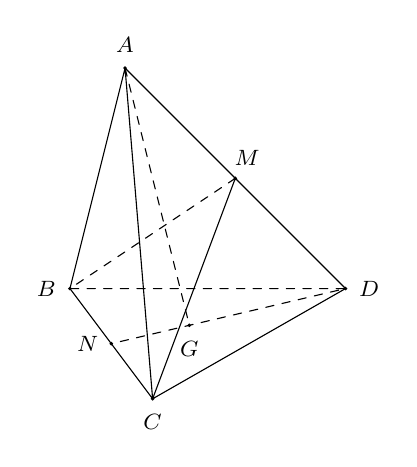
\begin{tikzpicture}[scale=0.7, font=\footnotesize, line join=round, line cap=round, >=stealth]
		\path (0,0) coordinate(B)
		--+(1.5,-2)coordinate (C)
		--+(5,0) coordinate (D)
		--+(1,4) coordinate (A)
		(A)--(D) coordinate[pos=0.5](M)
		(B)--(C) coordinate[pos=0.5](N)
		(D)--(N) coordinate[pos=2/3](G)
		;
		\draw (B)--(C)--(D)--(A)--cycle (A)--(C)--(M);
		\draw[dashed] (M)--(B)--(D)--(N) (A)--(G);
		\foreach \p/\q in {B/180,C/-90,D/0,A/90,M/60,N/180,G/-90}{
			\path (\p) node[shift={(\q:3mm)}]{$\p$};
			\fill[black] (\p) circle (1pt);}
		\end{tikzpicture}}
	\loigiai{
		\immini{
			Trong mặt phẳng $(AND)$ gọi $K = MN \cap AG$.\\
			Ta có $K\in AG$. \quad (1)\\ 
			và $K\in MN$, $MN \subset (BCM)\Rightarrow K \in (BCM)$. \quad (2)\\
			Từ $(1)$ và $(2)$ ta suy ra $K= AG \cap (BCM)$.
		}{
			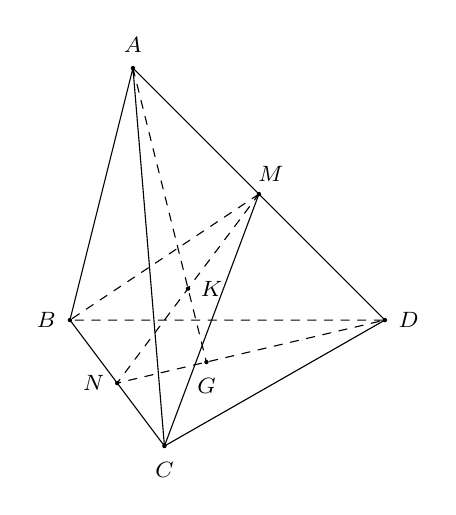
\begin{tikzpicture}[scale=0.8, font=\footnotesize, line join=round, line cap=round, >=stealth]
			\path (0,0) coordinate(B)
			--+(1.5,-2)coordinate (C)
			--+(5,0) coordinate (D)
			--+(1,4) coordinate (A)
			(A)--(D) coordinate[pos=0.5](M)
			(B)--(C) coordinate[pos=0.5](N)
			(D)--(N) coordinate[pos=2/3](G)
			(intersection of M--N and A--G) coordinate(K)
			;
			\draw (B)--(C)--(D)--(A)--cycle (A)--(C)--(M);
			\draw[dashed] (M)--(B)--(D)--(N) --(M) (A)--(G) ;
			\foreach \p/\q in {B/180,C/-90,D/0,A/90,M/60,N/180,G/-90,K/0}{
				\path (\p) node[shift={(\q:3mm)}]{$\p$};
				\fill[black] (\p) circle (1pt);}
			\end{tikzpicture}
		}
	}
\end{ex}

\begin{ex}%[1H4H1-3]%[Dự án đề cương 2025]%[Trịnh Văn Cảnh]
	Cho hình chóp $S.ABCD$ có đáy $ABCD$ là hình bình hành, $M$ và $N$ lần lượt là trung điểm của các cạnh $SD$ và $BC$. Giao tuyến của mặt phẳng $(DMN)$ và $(SAB)$ là.
	\choice
	{\True $SI$ với $I$ là giao điểm của $AB$ và $DN$}
	{$SI$ với $I$ là giao điểm của $SB$ và $MN$}
	{$SD$}
	{$SI$ với $I$ là giao điểm của $DN$ và $SB$}
	\loigiai{\immini{Ta có $S\in DM\Rightarrow S\in (DMN)$, $\Rightarrow S\in (DMN)\cap (SAB).\qquad (1)$\\
	Gọi $I$ là giao điểm của $DN$ và $AB$, khi đó do $I\in DM$ nên $I\in (DMN)$. Tương tự ta có $I\in (SAB).\qquad (2)$\\
	Từ $(1)$ và $(2)$ ta suy ra $SI$ là giao tuyến của hai mặt phẳng $(DMN)$ và $(SAB)$.}{
			\begin{tikzpicture}[scale=1,font=\footnotesize,line join=round,line cap=round,>=stealth] 
			\path 
			(0,0) coordinate (A) 
			(-1,-1) coordinate (B) 
			($(A)+(3,0)$) coordinate (D) 
			($(B)+(3,0)$) coordinate (C) 
			($(A)+(0.5,2)$) coordinate (S)
			($(S)!0.5!(D)$) coordinate (M)
			($(B)!0.5!(C)$) coordinate (N)
			(intersection of A--B and D--N) coordinate (I); 
			\draw (S)--(I)--(N)--(C)--(S)--(D)--(C);
			\draw[dashed] (I)--(B)--(S)--(A)--(B)--(N)--(M) (A)--(D)--(N); 
			\foreach \p/\g in {S/135,A/135,B/-45,C/-45,D/45,M/45,N/-45,I/-90} 
			\fill[black](\p) circle (1pt) ($(\p)+(\g:3mm)$) node{$\p$}; 
			\end{tikzpicture}}
	}
\end{ex}

\begin{ex}%[1H4H1-4]%[Dự án đề cương 2025]%[Trịnh Văn Cảnh] 
	Cho hình chóp $S.ABCD$, có đáy $ABCD$ là hình thang đáy lớn $AB$. Khi đó giao điểm của $BC$ và $(SAD)$ là 
	\choice
	{giao điểm của $BC$ với $SA$}
	{giao điểm của $BC$ với $SD$}
	{\True giao điểm của $BC$ với $AD$}
	{giao điểm của $AC$ với $BD$}
	\loigiai{\immini{
			\begin{itemize}
				\item Trong mặt phẳng $(ABCD)$, gọi $I=AD\cap BC$.
				\item Khi đó $\heva{&I\in BC\\&I\in AD\subset (SAD)}\Rightarrow BC\cap (SAD)=I$.
			\end{itemize}
		}{
			\begin{tikzpicture}[scale=1,font=\footnotesize,line join=round,line cap=round,>=stealth] 
			\path 
			(0,0) coordinate (A) 
			(4,0) coordinate (B) 
			(2.5,-1) coordinate (C) 
			(1,-1) coordinate (D) 
			(1,2) coordinate (S)
			(intersection of A--D and B--C) coordinate (I);
			\draw[dashed] (A)--(B); 
			\draw (I)--(D)--(S)--(A)--(D)--(C)--(B)--(S)--(C)--(I); 
			\foreach \p/\g in {S/135,A/180,B/0,C/-45,D/-135,I/-90} 
			\fill[black](\p) circle (1pt) ($(\p)+(\g:3mm)$) node{$\p$}; 
			\end{tikzpicture}}	
	}
\end{ex}

\begin{ex}%[1H4H1-4]%[Dự án đề cương 2025]%[Trịnh Văn Cảnh] 
	Cho hình chóp $S.ABCD$, có đáy $ABCD$ là hình bình hành tâm $O$. Khi đó giao điểm $I$ của $AM$ và $(SBD)$ là
	\choice
	{\True trọng tâm của tam giác $SAC$}
	{trung điểm của $AM$}
	{trung điểm của $SO$}
	{trọng tâm của tam giác $SCD$}
	\loigiai{
		\immini
		{
			\begin{itemize}
				\item Trong mặt phẳng $(SAC)$, gọi $I=AM\cap SO$.
				\item Khi đó $\heva{&I\in AM\\&I\in SO\subset (SBD)}\Rightarrow AM\cap (SBD)=I$.
				\item Trong tam giác $SAC$ do $AM$ và $SO$ là các đường trung tuyến nên $I$ là trọng tâm của tam giác $SAC$.
			\end{itemize}
		}{
			\begin{tikzpicture}[scale=1,font=\footnotesize,line join=round,line cap=round,>=stealth] 
			\path 
			(0,0) coordinate (A) 
			(-1,-1) coordinate (B) 
			($(A)+(3,0)$) coordinate (D) 
			($(B)+(3,0)$) coordinate (C) 
			($(A)+(0.5,2)$) coordinate (S)
			($(S)!0.5!(C)$) coordinate (M)
			(intersection of A--C and B--D) coordinate (O)
			(intersection of A--M and S--O) coordinate (I); 
			\draw[dashed] (S)--(A)--(C) (M)--(A)--(B)--(D)--(A) (S)--(O); 
			\draw (S)--(B)--(C)--(D)--(S)--(C); 
			\foreach \p/\g in {S/135,A/135,B/-135,C/-45,D/45,O/-90,M/30,I/135} 
			\fill[black](\p) circle (1pt) ($(\p)+(\g:3mm)$) node{$\p$}; 
			\end{tikzpicture}}	
	}
\end{ex}

\begin{ex}%[1H4H1-4]%[Dự án đề cương 2025]%[Trịnh Văn Cảnh] 
	Cho tứ diện $ABCD$. Gọi $E$ và $F$ lần lượt là trung điểm của $AB$ và $CD$; $G$ là trọng tâm tam giác $BCD$. Giao điểm của đường thẳng $EG$ và mặt phẳng $(ACD)$ là
	\choice
	{Giao điểm của đường thẳng $EG$ và $CD$}
	{Giao điểm của đường thẳng $EG$ và $AC$}
	{\True Giao điểm của đường thẳng $EG$ và $AF $}
	{Điểm $F $}
	\loigiai
	{
		\immini
		{
			\begin{itemize}
				\item Vì $G$ là trọng tâm tam giác $BCD$ và $F$ là trung điểm của $CD$ nên suy ra $G\in (ABF)$.
				\item Ta có $E$ là trung điểm của $AB\Rightarrow E\in (ABF)$.
				\item Gọi $M$ là giao điểm của $EG$ và $AF$ mà $AF\subset (ACD)$ nên $M\in (ACD)$.
				\item Vậy giao điểm của $EG$ và $(ACD)$ là $M=EG\cap AF$.
			\end{itemize}
		}{
			\begin{tikzpicture}[scale=1,font=\footnotesize,line join=round,line cap=round,>=stealth] 
			\path 
			(0,0) coordinate (B) 
			(1.5,-1.5) coordinate (C) 
			(5,0) coordinate (D) 
			(2,3) coordinate (A)
			($(A)!0.5!(B)$) coordinate (E)
			($(C)!0.5!(D)$) coordinate (F)
			($(B)!2/3!(F)$) coordinate (G)
			(intersection of E--G and A--F) coordinate (M)
			(intersection of E--M and C--D) coordinate (I); 
			\draw (A)--(B)--(C)--(D)--(A)--(C) (A)--(M)--(I); 
			\draw[dashed] (D)--(B)--(F) (E)--(I); 
			\foreach \p/\g in {A/90,B/180,C/-90,D/0,E/135,F/0,G/-120,M/0} 
			\fill[black](\p) circle (1pt) ($(\p)+(\g:3mm)$) node{$\p$};
			\path 
			(A)--(E) node[pos=0.5,sloped,scale=0.5]{$/$}
			(B)--(E) node[pos=0.5,sloped,scale=0.5]{$/$}
			(C)--(F) node[pos=0.5,sloped,scale=0.5]{$//$}
			(D)--(F) node[pos=0.5,sloped,scale=0.5]{$//$}; 
			\end{tikzpicture}}
	}
\end{ex}

\begin{ex}%[1H4H1-6]%[Dự án đề cương 2025]%[Trịnh Văn Cảnh]
	Cho hình tứ diện $ABCD$ có $M$, $N$ lần lượt là trung điểm của $AB$, $BD$. Các điểm $G$, $H$ lần lượt trên cạnh $AC$, $CD$ sao cho $NH$ cắt $MG$ tại $I$. Khẳng định nào sau đây là khẳng định đúng?
	\choice
	{$A$, $C$, $I$ thẳng hàng}
	{\True $B$, $C$, $I$ thẳng hàng}
	{$N$, $G$, $H$ thẳng hàng}
	{$B$, $G$, $H$ thẳng hàng}
	\loigiai{\immini{
			Do $NH$ cắt $MG$ tại $I$ nên bốn điểm $M$, $N$, $H$, $G$ cùng thuộc mặt phẳng $(\alpha)$.\\
			Ta có $\heva{&(\alpha) \cap(ABC)=MG\\
				&(\alpha) \cap(BCD)=NH\\
				&(ABC) \cap(BCD)=BC}$ mà $MG\cap NH=I$.\\			
			Suy ra $MG$, $NH$, $BC$ đồng quy tại $I$ nên $B$, $C$, $I$ thẳng hàng.}{\begin{tikzpicture}[scale=1,font=\footnotesize,line join=round,line cap=round,>=stealth]
			\path
			(0,0) coordinate (B)
			(1,-2) coordinate (C)
			(4,0) coordinate (D)
			(1.5,3.4)coordinate (A)
			($(A)!0.5!(B)$) coordinate (M)
			($(B)!.5!(D)$) coordinate (N)
			($(A)!2/3!(C)$) coordinate (G)
			($(D)!2/3!(C)$) coordinate (H)
			(intersection of N--H and M--G) coordinate (I)
			;
			\draw (D)--(A)--(B)--(C)--(I) (H)--(D)(A)--(C) (H)--(I) (M)--(I);
			\draw[dashed] (B)--(D) (M)--(N)--(H)--(C);
			\foreach \p/\q in {A/90,B/180,C/-120,D/0,M/140,N/30,I/-90,G/0,H/-30}
			\fill[black] (\p) circle (1.0pt) ($(\p)+(\q:2.5mm)$) node{$\p$};
			\end{tikzpicture}}}
\end{ex}
\begin{ex}%[1H4H1-6]%[Dự án đề cương 2025]%[Trịnh Văn Cảnh]
	Cho hình chóp $S.ABCD$. Một mặt phẳng $(P)$ bất kỳ cắt các cạnh $SA$, $SB$, $SC$, $SD$ lần lượt tại $A'$, $B'$, $C'$, $D'$. Gọi $I$ là giao điểm của $AC$ và $BD$. Chọn khẳng định đúng trong các khẳng định dưới đây:
	\choice
	{Các đường thẳng $AB$, $CD$, $C'D'$ đồng quy}
	{Các đường thẳng $AB$, $CD$, $A'B'$ đồng quy}
	{\True Các đường thẳng $A'C'$, $B'D'$, $SI$ đồng quy}
	{Các đường thẳng $SB$, $AD$, $B'C'$ đồng quy}
	\loigiai{
		\immini{
			Hai mặt phẳng $(P)$ và $(SAC)$ cắt nhau theo giao tuyến $A'C'$.\\
			Hai mặt phẳng $(P)$ và $(SBD)$ cắt nhau theo giao tuyến $B'D'$.\\
			Hai mặt phẳng $(SAC)$ và $(SBD)$ cắt nhau theo giao tuyến $SI$.\\
			Vậy ba đường thẳng $A'C'$, $B'D'$, $SI$ đồng quy.
		}{
			\begin{tikzpicture}[>=stealth,line join=round,line cap=round,font=\footnotesize,scale=.8]
			\tikzset{
				pics/hinhChopTuGiacthuong/.style  n args={5}{
					code={
						\tikzset{
							declare function={a=4;b=2;h=3;goc=-130;goc2=-40;c=3.5;}
						}	
						\path 
						(0,0)coordinate (#1)+(0:a)coordinate (#2)+(goc:b)coordinate (#4)+(80:h)coordinate (#5)+(goc2:c)coordinate (#3)		
						;
					}
			}}
			\path 
			(0,0)pic {hinhChopTuGiacthuong={A}{B}{C}{D}{S}}
			(intersection of A--C and B--D)coordinate (I)
			($(S)!.5!(A)$)coordinate (A')
			($(S)!.6!(D)$)coordinate (D')
			($(S)!.5!(C)$)coordinate (C')
			(intersection of A'--C' and S--I)coordinate (I1)
			(intersection of D'--I1 and S--B)coordinate (B')
			;	
			
			\foreach \pointo/\pointt in {S/B,S/C,S/D,B/C,C/D,B'/C',C'/D'}{
				\draw[fill=black](\pointo)--(\pointt);
			}
			\foreach \pointo/\pointt in {S/A,A/B,A/D,A/C,B/D,S/I,A'/B',A'/D',A'/C',B'/D'}{
				\draw[fill=black,dashed](\pointo)--(\pointt);
			}
			\foreach \point/\goc in {S/90,A/150,B/10,C/-20,D/190,I/-90,A'/130,B'/45,C'/-25,D'/180}{
				\draw[fill=black](\point)circle(.8pt)+(\goc:2mm)node[scale=.8]{$\point$};
			}
			\end{tikzpicture}
		}
		
	}
\end{ex}
\begin{ex}%[1H4H1-3]%[Dự án đề cương 2025]%[Trịnh Văn Cảnh]
	\immini{Cho hình chóp $S.ABCD$ có đáy là hình thang với đáy lớn $AB$. Gọi $M$ là trung điểm $SC$. Tìm giao tuyến của mặt phẳng $(MAD)$ và $(SBC)$.
		\choice
		{$ME$ (với $E$ là giao điểm của $AB$ và $CD$)}
		{\True $ME$ (với $E$ là giao điểm của $AD$ và $BC$)}
		{$SE$ (với $E$ là giao điểm của $AB$ và $CD$)}
		{ $SE$ (với $E$ là giao điểm của $AD$ và $BC$)}}{
		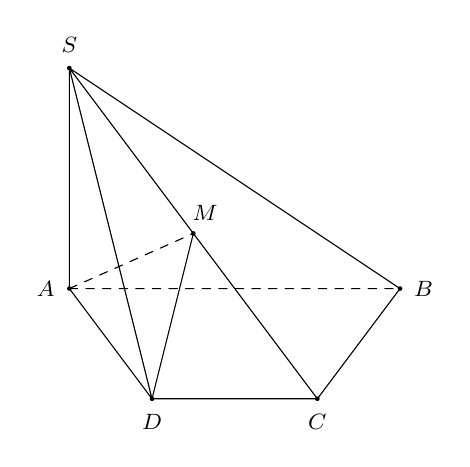
\begin{tikzpicture}[scale=0.7, font=\footnotesize, line join=round, line cap=round, >=stealth]
		\path (0,0)coordinate(A)
		--++(1.5,-2) coordinate(D)
		--++(3,0) coordinate(C)
		(A)--+(6,0) coordinate (B)
		--+(0,4) coordinate (S)
		(S)--(C) coordinate[pos=0.5](M);
		\draw (S)--(D)--(C)--(B)--cycle (S)--(C) (S)--(A) (A)--(D)--(M);
		\draw[dashed] (A)--(B) (A)--(M);
		\foreach \p/\q in {A/180,D/-90,C/-90,B/0,S/90,M/60}{
			\path (\p) node[shift={(\q:3mm)}]{$\p$};
			\fill[black] (\p) circle (1.2pt);}
		\end{tikzpicture} }
	\loigiai{
		\immini{Ta có $M\in (MAD)$.\\
			Mặt khác $M\in SC$, $SC\subset (SBC) \Rightarrow M\in (SBC)$ nên $M$ là điểm chung thứ nhất của hai mặt phẳng $(SBC)$ và $(MAD)$.\\
			Trong mặt phẳng $(ABCD)$ gọi $E = AD \cap BC\Rightarrow \heva{& E\in AD \\& E \in BC}\Rightarrow \heva{& E \in (MAD) \\& E \in (SBC)}$ suy ra $E$ là điểm chung thứ hai.\\
			Vậy $ME= (MAD)\cap (SBC)$.}{ 
			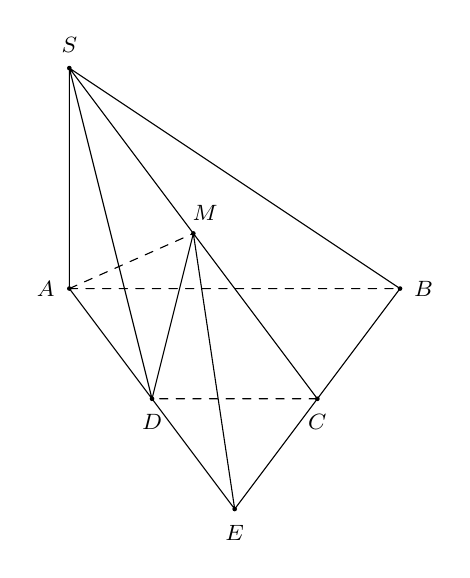
\begin{tikzpicture}[scale=0.7, font=\footnotesize, line join=round, line cap=round, >=stealth]
			\path (0,0)coordinate(A)
			--++(1.5,-2) coordinate(D)
			--++(3,0) coordinate(C)
			(A)--+(6,0) coordinate (B)
			--+(0,4) coordinate (S)
			(S)--(C) coordinate[pos=0.5](M)
			(intersection of A--D and B--C) coordinate(E)
			;
			\draw (D)--(S) --(B)--(C) (S)--(C) (S)--(A) (A)--(D) (D)--(E)--(C) (D)--(M)--(E);
			\draw[dashed] (A)--(B) (A)--(M) (C)--(D) ;
			\foreach \p/\q in {A/180,D/-90,C/-90,B/0,S/90,M/60,E/-90}{
				\path (\p) node[shift={(\q:3mm)}]{$\p$};
				\fill[black] (\p) circle (1.2pt);}
			\end{tikzpicture}
		}	
	}
\end{ex}

\begin{ex}%[1H4H1-4]%[Dự án đề cương 2025]%[Trịnh Văn Cảnh] 
	Cho tứ diện $ABCD$. Gọi $E$, $F$ lần lượt là trung điểm của $AB$ và $CD$; Gọi $M$ là trung điểm của $BF$ và $G$ là giao điểm của $AM$ và $(ECD)$. Khẳng định nào sau đây \textbf{đúng}?
	\choice
	{$G$ là trọng tâm của tam giác $ECD$}
	{$G$ là trọng tâm của tam giác $ABC$}
	{$G$ là trọng tâm của tam giác $ABD$}
	{\True $G$ là trọng tâm của tam giác $ABF$}
	\loigiai
	{
		\immini
		{
			\begin{itemize}
				\item Trong mặt phẳng $(ABF)$, gọi $G=AM\cap EF$.
				\item Khi đó $\heva{&G\in AM\\&G\in EF\subset (ECD)}\Rightarrow AM\cap (ECD)=G$.
				\item Vì $AM$ và $EF$ là đường trung bình của tam giác $ABF$ nên suy ra $G$ là trọng tâm của tam giác $ABF$.
			\end{itemize}	
		}{
			\begin{tikzpicture}[scale=1,font=\footnotesize,line join=round,line cap=round,>=stealth] 
			\path 
			(0,0) coordinate (B) 
			(3,-1.5) coordinate (C) 
			(5,0) coordinate (D) 
			(2,3) coordinate (A)
			($(A)!0.5!(B)$) coordinate (E)
			($(C)!0.5!(D)$) coordinate (F)
			($(B)!0.5!(F)$) coordinate (M)
			(intersection of A--M and E--F) coordinate (G); 
			\draw (A)--(B)--(C)--(D)--(A)--(C)--(E) (A)--(F); 
			\draw[dashed] (F)--(B)--(D)--(E)--(F) (A)--(M); 
			\foreach \p/\g in {A/90,B/180,C/-90,D/0,E/135,F/-45,M/-135,G/-135} 
			\fill[black](\p) circle (1pt) ($(\p)+(\g:3mm)$) node{$\p$};
			\path 
			(A)--(E) node[pos=0.5,sloped,scale=0.5]{$/$} (B)--(E) node[pos=0.5,sloped,scale=0.5]{$/$}
			(C)--(F) node[pos=0.5,sloped,scale=0.5]{$//$} (D)--(F) node[pos=0.5,sloped,scale=0.5]{$//$}
			(B)--(M) node[pos=0.5,rotate=30,scale=0.5]{$/$} node[pos=0.51,rotate=-30,scale=0.5]{$/$}
			(M)--(F) node[pos=0.5,rotate=30,scale=0.5]{$/$} node[pos=0.51,rotate=-30,scale=0.5]{$/$}
			; 
			\end{tikzpicture}
		}	
	}
\end{ex}

\begin{ex}%[1H4H1-4]%[Dự án đề cương 2025]%[Trịnh Văn Cảnh] 
	Cho hình chóp $S.ABCD$, có đáy $ABCD$ là hình thang với đáy lớn là $AD$. Gọi $E$, $F$ lần lượt là hai điểm nằm trên hai cạnh $SB$ và $CD$. Khi đó giao điểm của $SC$ và $(AEF)$ là 
	\choice
	{giao điểm của $SC$ và $EM$, với $M=BF\cap AD$}
	{\True giao điểm của $SC$ và $EM$, với $M=AF\cap BC$}
	{giao điểm của $SC$ và $EM$, với $M=AC\cap BD$}
	{giao điểm của $SC$ và $EM$, với $E=BF\cap AC$}
	\loigiai
	{
		\immini
		{
			\begin{itemize}
				\item Trong mặt phẳng $(ABCD)$, gọi $M=AF\cap BC$.
				\item Trong mặt phẳng $(SBC)$, gọi $I=SC\cap EM$.
				\item Khi đó $\heva{&I\in SC\\&I\in EM\subset (AEF)}\Rightarrow SC\cap (AEF)=I$.
			\end{itemize}
		}{
			\begin{tikzpicture}[scale=1,font=\footnotesize,line join=round,line cap=round,>=stealth] 
			\path 
			(0,0) coordinate (A) 
			(1,-1.5) coordinate (B) 
			(3,-1.5) coordinate (C)
			(5,0) coordinate (D) 
			(2,3) coordinate (S)
			($(S)!0.4!(B)$) coordinate (E)
			($(C)!0.3!(D)$) coordinate (F)
			(intersection of A--F and B--C) coordinate (M)
			(intersection of S--C and E--M) coordinate (I)
			(intersection of E--M and C--D) coordinate (J);
			\draw[dashed] (A)--(D) (A)--(F)--(E) (C)--(J) (F)--(M); 
			\draw (B)--(S)--(A)--(B)--(C)--(S)--(D)--(J) (A)--(E)--(M)--(C); 
			\foreach \p/\g in {S/135,A/180,B/-135,C/-45,D/0,E/135,F/-60,M/45,I/45} 
			\fill[black](\p) circle (1pt) ($(\p)+(\g:3mm)$) node{$\p$}; 
			\end{tikzpicture}}	
	}
\end{ex}
\begin{ex}%[1H4H1-4]%[Dự án đề cương 2025]%[Trịnh Văn Cảnh] 
	Cho tứ diện $ABCD$. Gọi $M$ là trung điểm của $AB$ và $N$ là điểm trên cạnh $AD$ sao cho $AN=2ND$. Khi đó giao điểm $E$ của $MN$ và $(BCD)$ là
	\choice
	{\True điểm đối xứng với $B$ qua $D$}
	{điểm đối xứng với $B$ qua $C$}
	{điểm đối xứng với $D$ qua $B$}
	{điểm đối xứng với $C$ qua $B$}
	\loigiai{
		\immini
		{
			\begin{itemize}
				\item Trong mặt phẳng $(ABD)$, gọi $E=MN\cap BD$.
				\item Khi đó $\heva{&E\in MN\\&E\in BD\subset (BCD)}\Rightarrow MN\cap (BCD)=E$.
				\item Dễ thấy trong tam giác $ABE$ có $EM$ và $AD$ là các đường trung tuyến nên $N$ là trọng tâm của tam giác $ABE$ suy ra $D$ là trung điểm của $AE$.
				\item Do đó $E$ là điểm đối xứng với $B$ qua $D$.
			\end{itemize}
		}{
			\begin{tikzpicture}[scale=1,font=\footnotesize,line join=round,line cap=round,>=stealth] 
			\path 
			(0,0) coordinate (B) 
			(1.5,-1.5) coordinate (C) 
			(3,0) coordinate (D) 
			(2,2) coordinate (A)
			($(A)!0.5!(B)$) coordinate (M)
			($(A)!2/3!(D)$) coordinate (N)
			(intersection of M--N and B--D) coordinate (E); 
			\draw (A)--(B)--(C)--(D)--(A)--(C) (D)--(E)--(N); 
			\draw[dashed] (D)--(B) (M)--(N); 
			\foreach \p/\g in {A/90,B/180,C/-90,D/45,M/135,N/45,E/90} 
			\fill[black](\p) circle (1pt) ($(\p)+(\g:3mm)$) node{$\p$};
			\path 
			(A)--(M) node[pos=0.5,sloped,scale=0.5]{$/$}
			(B)--(M) node[pos=0.5,sloped,scale=0.5]{$/$}; 
			\end{tikzpicture}}	
	}
\end{ex}

\Closesolutionfile{ans}

\ind{PHẦN II.} \inden{Câu trắc nghiệm đúng sai. Trong mỗi ý a), b), c), d) ở mỗi câu, học sinh chọn đúng hoặc sai.}\\
\setcounter{ex}{0}
\Opensolutionfile{ans}[ans/2D1-Bai1-DS]%--Đặt tên 2D1-Bai1-DS
\begin{ex}%[1H4H1-4]%[Dự án đề cương 2025]%[Trịnh Văn Cảnh]
	Cho hình chóp $S.ABCD$, đáy là tứ giác lồi $ABCD$ có các cạnh đối không song song với nhau. Gọi $M$ là điểm trên cạnh $SA$, $O$ là giao điểm của $AC$ và $BD$. 
	\choiceTF[1t]
	{\True Giao tuyến của $(SAC)$ và $(SBD)$ là $SO$}
	{\True Giao tuyến của $(SAB)$ và $(SCD)$ là $SF$, với $F$ là giao điểm của $AB$ và $CD$}
	{Giao tuyến của $(SBC)$ và $(SAD)$ là $SM$}
	{\True Giao tuyến của $(BCM)$ và $(SAD)$ là $ME$, với $E$ là giao điểm của $AD$ và $BC$}
	\loigiai{\centerline{
			\begin{tikzpicture}[line cap=round,line join=round,font=\footnotesize]
			\path (0:0) coordinate(A) (0:4) coordinate(D) (-65:2.4) coordinate(B) ++(20:2.3) coordinate(C) (50:3) coordinate(S);
			\path ($(S)!.4!(A)$) coordinate(M) (intersection of A--C and B--D) coordinate(O) (intersection of A--D and B--C) coordinate(E) (intersection of A--B and C--D) coordinate(F);
			\draw (S)--(A)--(F)--cycle (S)--(C)--(E)--cycle (C)--(F) (S)--(B)--(M);
			\draw[dashed] (S)--(D)--(C)--(A)--(E) (C)--(B)--(D) (S)--(O)--(M)--(C) (M)--(E);
			\foreach \d/\g in {A/180, B/-135, C/-45, D/-45, S/90, O/-95, M/150, E/0, F/-90}
			\fill (\d) circle(1pt) node[shift={(\g:.3)}]{$\d$};
			\end{tikzpicture}}
		\begin{itemchoice}
			\itemch Ta có $S\in (SAC)\cap (SBD)$.\\
			Trong mặt phẳng $(ABCD)$, ta có $AC\cap BD =O$, $AC\subset (SAC)$, $BD\subset (SBD)$ nên $O\in (SAC)\cap (SBD)$.\\
			Vậy giao tuyến của $(SAC)$ và $(SBD)$ là $SO$.
			\itemch Ta có $S\in (SAB)\cap (SCD)$.\\
			Trong mặt phẳng $(ABCD)$, gọi $AB\cap CD =F$, mà $AB\subset (SAB)$, $CD\subset (SCD)$ nên $F\in (SAB)\cap (SCD)$.\\
			Vậy giao tuyến của $(SAB)$ và $(SCD)$ là $SF$.
			\itemch Ta có $S\in (SBC)\cap (SAD)$.\\
			Trong mặt phẳng $(ABCD)$, gọi $BC\cap AD = E$, mà $BC\subset (SBC)$, $AD\subset (SAD)$ nên $E\in (SBC)\cap (SAD)$.\\
			Vậy giao tuyến của $(SBC)$ và $(SAD)$ là $SE$, không phải $SM$.
			\itemch Ta có $M\in (BCM)\cap (SAD)$.\\
			Trong mặt phẳng $(ABCD)$, gọi $BC\cap AD = E$, mà $BC\subset (BCM)$, $AD\subset (SAD)$ nên $E\in (BCM)\cap (SAD)$.\\
			Vậy giao tuyến của $(BCM)$ và $(SAD)$ là $ME$.
		\end{itemchoice}
	}
\end{ex}

\begin{ex}%[1H4V1-6]%[Dự án đề cương 2025]%[Trịnh Văn Cảnh]
	Cho tứ diện $ABCD$. Gọi các điểm $E$, $F$, $G$ lần lượt thuộc các cạnh $AB$, $AC$, $BD$ sao cho $EF$ cắt $BC$ tại $I$, $EG$ cắt $AD$ tại $H$.
	\choiceTF[1t]
	{\True Ba đường thẳng $AB$, $IF$, $HG$ đồng quy tại $E$}
	{Ba điểm $H$, $I$, $G$ thẳng hàng}
	{Hai đường thẳng $CD$ và $FG$ cắt nhau}
	{\True Ba đường thẳng $HF$, $IG$, $CD$ đồng quy}
	\loigiai
	{
		\centerline
		{
			\begin{tikzpicture}[line cap=round,line join=round,font=\footnotesize]
			\path (0:0) coordinate(B) (0:4) coordinate(C) (-30:3) coordinate(D) (55:3.2) coordinate(A) ($(A)!.4!(B)$) coordinate(E) ($(A)!.7!(C)$) coordinate(F) ($(B)!.8!(D)$) coordinate(G);
			\path (intersection of E--F and B--C) coordinate(I) (intersection of E--G and A--D) coordinate(H) (intersection of H--F and D--C) coordinate(J);
			\draw (A)--(B)--(D)--cycle (I)--(F)--(H)--cycle (A)--(H)--(E) (I)--(J) (A)--(F) (D)--(J);
			\draw[dashed] (B)--(I) (E)--(F) (G)--(J) (F)--(C)--(J);
			\foreach \d/\g in {A/90, B/180, C/-45, D/-10, E/120, F/45, G/7-145, I/0, H/-90, J/-50}
			\fill (\d) circle(1pt) node[shift={(\g:.3)}]{$\d$};
			\end{tikzpicture}
		}
		\begin{itemchoice}
			\itemch Vì $\left\{\begin{aligned}&E\in AB \\&E\in IF \\&E\in HG\end{aligned}\right.$ nên ba đường thẳng $AB$, $IF$, $HG$ đồng quy tại $E$.
			\itemch Sai. Vì $H$, $I$, $G$ không cùng nằm trên một đường thẳng, hay nói cách khác $H$, $I$, $G$ không cùng nằm trên giao tuyến chung của hai mặt phẳng nào.
			\itemch Sai. Vì $CD$ và $FG$ nằm trên hai mặt phẳng khác nhau nên không có điểm chung.
			\itemch Ta có $IG$ và $CD$ cùng chứa trong mặt phẳng $(BCD)$, ta gọi $J=IG\cap CD$.\\
			Vì $F=EI\cap AC$, $EI\subset (EIH)$, $AC\subset (ACD)$ nên $F\in (EIH)\cap (ACD)$.\\
			Vì $H=EG\cap AD$, $EG\subset (EIH)$, $AD\subset (ACD)$ nên $H\in (EIH)\cap (ACD)$.\\
			Do đó, $(EIH)\cap (ACD) = FH$.\\
			Lại có $\left\{\begin{aligned}&J\in IG; IG\subset (EIH) \\&J\in CD; CD\subset (ACD)\end{aligned}\right.$ nên $J\in (EIH)\cap (ACD)$ hay $J\in FH$.\\
			Vậy ba đường thẳng $HF$, $IG$, $CD$ đồng quy tại $J$.
		\end{itemchoice}
	}
\end{ex}
\begin{ex}%[1H4H1-6]%[Dự án đề cương 2025]%[Trịnh Văn Cảnh]
	Cho hình bình hành $ABCD$ và một điểm $S$ không thuộc mặt phẳng $(ABCD)$, các điểm $M$, $N$ lần lượt là trung điểm của đoạn thẳng $AB$, $SC$. Gọi $O=AC \cap BD$; 
	\choiceTF[t]
	{\True $SO$ giao tuyến của hai mặt phẳng $(SAC)$ và $(SBD)$}
	{\True Giao điểm của $I$ của đường thẳng $AN$ và mặt phẳng $(SBD)$ là điểm nằm trên đường thẳng $SO$}
	{Giao điểm của $J$ của đường thẳng $MN$ và mặt phẳng $(SBD)$ là điểm nằm trên đường thẳng $SD$}
	{\True Ba điểm $I$, $J$, $B$ thẳng hàng}
	\loigiai{
		\begin{center}
			\begin{tikzpicture}[scale=1.1, font=\footnotesize, line join=round, line cap=round,>=stealth]
			\path
			(0,0) coordinate (A)
			(1.3,-2.1) coordinate (B)
			(4.8,-2.1)coordinate (C)
			($(A)+(C)-(B)$) coordinate (D)
			($(D)+(-0.5,3.2)$) coordinate (S)
			(intersection of A--C and B--D) coordinate (O)
			($(A)!0.5!(B)$) coordinate (M)
			($(S)!0.5!(C)$) coordinate (N)	
			(intersection of C--M and B--D) coordinate (P)	
			(intersection of A--N and S--O) coordinate (I)	
			(intersection of M--N and S--P) coordinate (J)		
			;
			\draw (S)--(A)--(B)--(C)--cycle (S)--(B);
			\draw[dashed] (O)--(S)--(D)--(B)--(A)--(C)--(D)--(A)--(N)--(M)--(C)
			(P)--(S);	
			\foreach \p/\q in {S/90,A/180,B/-90,C/-90,D/0,O/-90,M/220,N/30, P/-90,I/40,J/160}			
			\fill[black] (\p) circle (1.0pt)node[shift={(\q:3mm)}]{$\p$};
			\end{tikzpicture}
		\end{center}
		\begin{itemchoice}
			\itemch $SO$ giao tuyến của hai mặt phẳng $(SAC)$ và $(SBD)$.
			\itemch Tìm giao điểm $I$ của $AN$ và mặt phẳng $(SBD)$.\\
			Trong mặt phẳng $(ABCD)$, gọi $O=AC \cap BD$;\\
			Trong mặt phẳng $(SAC)$, gọi $I=SO \cap AN$.\\
			Ta có $\heva{& I\in AN \\	& I \in SO, SO \subset(SBD)} 
			\Rightarrow I=AN \cap(SBD)$.		
			\itemch Tìm giao điểm $J$ của $MN$ và mặt phẳng $(SBD)$.\\		
			Trong mặt phẳng $(ABCD)$, gọi $P=C M \cap BD$;\\
			Trong mặt phẳng $(SCM)$, gọi $J=MN \cap S P$;\\
			Ta có $\heva{& J \in MN \\& J \in SP, SP \subset(SBD)} 
			\Rightarrow J=MN \cap(SBD)$.
			\itemch Chứng minh $I$, $J$, $B$ thẳng hàng.\\
			Dễ thấy $B \in(ABN) \cap(SBD).\quad (1)$\\
			Ta có $\heva{& I \in AN, A N \subset(ABN) \\& I \in SO, SO \subset(SBD)} 
			\Rightarrow I \in(ABN) \cap(SBD).\quad(2)$\\
			Tương tự: $\heva{& J \in MN, MN \subset(ABN)\\& J \in S P, S P \subset(SBD)} \Rightarrow J \in(ABN) \cap(SBD).\quad(3)$\\
			Từ $(1)$, $(2)$, và $(3)$ suy ra $B$, $I$, $J$ cùng thuộc giao tuyến của hai mặt phẳng $(ABN)$ và $(SBD)$ nên ba điểm này thẳng hàng.
		\end{itemchoice}
	}
\end{ex}
\begin{ex}%[1H4V1-4]%[Dự án đề cương 2025]%[Trịnh Văn Cảnh]
	Cho hình chóp $S.ABCD$ có $ABCD$ là hình thang đáy lớn $AD$ và $AD=2BC$. Gọi $O=AC\cap BD$, $M$ là điểm thuộc cạnh $SD$ sao cho $SM=2MD$.
	\choiceTF[t]
	{\True Đường thẳng $AC$ cắt mặt phẳng $(SBD)$ tại $O$}
	{\True Đường thẳng $BM$ cắt mặt phẳng $(SAC)$ tại $I$, với $I$ là giao điểm của $BM$ và $SO$}
	{Đường thẳng $SB$ cắt mặt phẳng $(MAC)$ tại $N$, với $N$ là giao điểm của $CM$ và $SB$}
	{\True Đường thẳng $SB$ cắt mặt phẳng $(MAC)$ tại $N$, khi đó tỉ số $\dfrac{SN}{SB}=\dfrac{4}{3}$}
	\loigiai{
		\begin{center}
			\begin{tikzpicture}[scale=1, line join=round, line cap=round, >=stealth]
			\coordinate (A) at (0,0);
			\coordinate (B) at (-2,-1.5);
			\coordinate (C) at (1,-1.5);
			\coordinate (d) at ($(C)-(B)+(A)$);
			\coordinate (D) at ($(A)!2!(d)$);
			\coordinate (S) at (0.3,3);
			\coordinate (O) at (intersection of A--C and B--D);
			\coordinate (M) at ($(S)!2/3!(D)$);
			\coordinate (I) at (intersection of B--M and S--O);
			\coordinate (N) at (intersection of S--B and M--O);
			\coordinate (n) at (intersection of B--C and M--N);
			\draw 
			(S)--(B)--(C)--(D)--(S)--(C)
			(B)--(N)--(n)
			;
			\draw[dashed] 
			(S)--(A)--(B)--(D)--(A)--(C)
			(B)--(M)--(n)
			(S)--(O)
			;
			\foreach \x/\g in {S/90,A/60,D/60,C/-70,B/-150,M/60,N/-90,O/-100,I/140} \fill[black](\x) circle (1pt)+(\g:0.3)node{$\x$};
			\end{tikzpicture}
			\begin{tikzpicture}[scale=1, line join=round, line cap=round, >=stealth]
			\coordinate (S) at (3,4);
			\coordinate (B) at (0,0);
			\coordinate (D) at (6,0);
			\coordinate (O) at ($(B)!1/3!(D)$);
			\coordinate (K) at ($(B)!2/3!(D)$);
			\coordinate (M) at ($(S)!2/3!(D)$);
			\coordinate (N) at (intersection of M--O and S--B);
			\draw 
			(S)--(B)--(D)--(S)--(O)
			(B)--(N)--(M)--(K)
			;
			\foreach \x/\g in {S/90,D/0,B/180,M/30,O/-90,K/-90,N/-90} \fill[black](\x) circle (1pt)+(\g:0.3)node{$\x$};
			\end{tikzpicture}
		\end{center}
		\begin{itemchoice}
			\itemch Ta có $O=AC\cap BD$, suy ra
			\[\heva{& O \in BD \Rightarrow O \in(SBD) \\
				& O \in AC} \Rightarrow AC \cap(SBD)=O.\]
			\itemch Trong $(SBD)$, gọi $I=BM \cap SO$. Ta có 
			\[\heva{& I \in BM \\ & I \in SO \subset(SAC) \Rightarrow I \in(SAC)} \Rightarrow BM \cap(SAC)=I.\]
			\itemch Dễ thấy $CM$ và $SB$ không cùng thuộc một mặt phẳng nên chúng không có điểm chung.
			\itemch Dễ thấy $OM=(SBD) \cap(MAC)$.\\
			Trong $(SBD)$, gọi $N=SB \cap OM$.\\
			Ta có $\heva{& N \in SB \\ & N \in OM} \Rightarrow \heva{& N \in SB \\ & N \in(MAC)} \Rightarrow N=SB \cap(MAC)$.\\
			Do $BC \parallel AD$ nên $\dfrac{OB}{OD}=\dfrac{OC}{OA}=\dfrac{BC}{AD}=\dfrac{1}{2} \Rightarrow OB=\dfrac{1}{3} BD$.\\
			Trong $(SBD)$, qua $M$ kẻ đường thẳng song song với $SB$, cắt $BD$ tại $K$.\\
			Suy ra $\dfrac{MK}{SB}=\dfrac{DK}{DB}=\dfrac{DM}{DS}=\dfrac{1}{3} \Rightarrow DK=\dfrac{1}{3} DB$ và $MK=\dfrac{1}{3} SB$.\\
			Trong $(SBD)$, ta có $MK \parallel SB \Rightarrow MK \parallel BN \Rightarrow \dfrac{BN}{KM}=\dfrac{OB}{OK}=1 \Rightarrow BN=KM=\dfrac{1}{3} SB$.\\
			Ta có $SN=SB+BN=SB+\dfrac{1}{3} SB=\dfrac{4}{3} SB$. Do đó $\dfrac{SN}{SB}=\dfrac{\dfrac{4}{3} SB}{SB}=\dfrac{4}{3}$.
		\end{itemchoice}		
	}
\end{ex}
\begin{ex}%[1H4V1-4]%[Dự án đề cương 2025]%[Trịnh Văn Cảnh]
	Cho hình chóp $S.ABCD$ có đáy $ABCD$ là hình bình hành tâm $O$. Gọi $M$ là trung điểm của $SC$, $N$ là trung điểm của $OB$ và $I$ là trọng tâm của tam giác $SAC$. Xét tính đúng, sai các khẳng định sau:
	\choiceTF[t]
	{Giao điểm của $SC$ và mặt phẳng $(AMN)$ là điểm $N$}
	{\True Giao điểm của $AM$ và mặt phẳng $(SBD)$ là điểm $I$}
	{Giao điểm của $NI$ và mặt phẳng $(SAD)$ là điểm $K$ thuộc đường thẳng $SA$}
	{Giao điểm của đường thẳng $SD$ và mặt phẳng $(AMN)$ là trung điểm của $SD$}
	\loigiai
	{
		\centerline
		{
			\begin{tikzpicture}[line cap=round,line join=round,font=\footnotesize]
			\path (0:0) coordinate(A) (45:2.3) coordinate(D) (0:4) coordinate(B) ($(B)+(D)-(A)$) coordinate(C) (65:5.5) coordinate(S) ($(B)!.5!(D)$) coordinate(O) ($(S)!.5!(C)$) coordinate(M) ($(B)!.5!(O)$) coordinate(N);
			\path (intersection of A--M and S--O) coordinate(I) (intersection of N--I and S--D) coordinate(K);
			\draw (S)--(A)--(B)--(C)--cycle (S)--(B);
			\draw[dashed] (S)--(D)--(B) (A)--(C)--(D)--cycle (A)--(M)--(N)--cycle (S)--(O) (N)--(K);
			\foreach \d/\g in {A/-135, B/-45, C/0, D/180, S/90, O/-95, M/45, N/-100, I/-10, K/10}
			\fill (\d) circle(1pt) node[shift={(\g:.3)}]{$\d$};
			\end{tikzpicture}
		}
		\begin{itemchoice}
			\itemch Ta có $SC\cap (AMN) = \{M\}$.
			\itemch Ta có $S\in (SAC)\cap (SBD)$.\\
			Trong mặt phẳng $(ABCD)$, ta có $AC\cap BD = \{O\}$, mà $AC\subset (SAC)$, $BD\subset (SBD)$ nên $O\in (SAC)\cap (SBD)$.\\
			Do đó, giao tuyến của hai mặt phẳng $(SAC)$ và $(SBD)$ là đường thẳng $SO$.\\
			Trong mặt phẳng $(SAC)$, gọi $AM\cap SO = \{J\}$.\\
			Khi đó $\left\{\begin{aligned}&J\in AM \\&J\in SO \\&SO\subset (SBD)\end{aligned}\right.$, suy ra $AM\cap (SBD) = \{J\}$.\\
			Mà $SO$, $AM$ là hai đường trung tuyến của tam giác $SAC$ nên $J$ là trọng tâm của tam giác $SAC$. Suy ra $J\equiv I$.\\
			Vậy giao điểm của $AM$ và mặt phẳng $(SBD)$ là điểm $I$.
			\itemch Trong mặt phẳng $(SBD)$, gọi $NI\cap SD = \{K\}$.\\
			Khi đó $\left\{\begin{aligned}&K\in NI \\&K\in SD \\&SD\subset (SAD)\end{aligned}\right.$, suy ra $NI\cap (SAD) = \{K\}$, với điểm $K$ thuộc đường thẳng $SD$.
			\itemch Trong mặt phẳng $(SBD)$, gọi $SD\cap NI = \{K\}$.\\
			Khi đó $\left\{\begin{aligned}&K\in SD \\&K\in NI \\&NI\subset (AMN)\end{aligned}\right.$, suy ra $SD\cap (AMN) = \{K\}$.\\
			Áp dụng định lí Menelaus cho tam giác $SOD$ và cát tuyến $KIN$ ta có
			\[\dfrac{KS}{KD}\cdot \dfrac{ND}{NO}\cdot \dfrac{IO}{IS} = 1 \Leftrightarrow \dfrac{KS}{KD} \cdot 3\cdot \dfrac{1}{2} = 1 \Leftrightarrow \dfrac{KS}{KD} = \dfrac{2}{3}.\]
			Vậy $K$ không là trung điểm của $SD$.
		\end{itemchoice}
	}
\end{ex}

\Closesolutionfile{ans}


\ind{PHẦN III.} \inden{Câu trắc nghiệm trả lời ngắn.}\\
\setcounter{ex}{0}
\Opensolutionfile{ans}[ans/2D1-Bai1-DS]%--Đặt tên 2D1-Bai1-DS

\begin{ex}%[1H4V1-6]%[Dự án đề cương 2025]%[Trịnh Văn Cảnh]
	Cho hình chóp $S.ABC$. Gọi $M$ là trung điểm đoạn $SA$. Điểm $N$ thuộc cạnh $SC$ sao cho $NS=2NC$. Gọi $E$ là giao điểm của $M N$ với mặt phẳng $(ABC)$. Tính $\dfrac{MN}{NE}$.
	\shortans{$0{,}5$}
	\loigiai{
		\immini{
			Trong $(SAC)$, ta có $\dfrac{SM}{MA}\ne\dfrac{SN}{NC}$ nên $MN$ và $AC$ cắt nhau. Khi đó giao điểm của $MN$ và $AC$ chính là giao điểm của $MN$ với mặt phẳng $(ABC)$. Do đó $E=MN\cap AC$.\\
			Xét tam giác $SAE$ có $EM$ là đường trung tuyến; $EM$ cắt $SC$ tại $N$ và $\dfrac{SN}{NC}=2$. Suy ra $N$ là trọng tâm của tam giác $SAE$.\\
			Vì vậy $\dfrac{MN}{NE}=\dfrac12=0{,}5$.
		}
		{
			\begin{tikzpicture}[scale=1, font=\footnotesize, line join=round, line cap=round, >=stealth]
			\def\bc{4} % cạnh BC
			\def\ba{2} % cạnh BA
			\def\h{4} % đường cao
			\def\gocB{125} % góc B của đáy
			\coordinate[label=below left:$B$] (B) at (0,0);
			\coordinate[label=left:$A$] (A) at (\gocB:\ba);
			\coordinate[label=above right:$C$] (C) at ($(A)+(4,0)$);
			
			\coordinate [label=above:$S$](S) at (70:5);
			\coordinate[label=left:$M$] (M) at ($(S)!1/2!(A)$);
			\coordinate[label=above right:$N$] (N) at ($(S)!2/3!(C)$);
			\path 
			(intersection of A--C and M--N) coordinate (E);
			\node at (E) [right]{$E$};
			\draw (S)--(A)--(B)--(E)--(N)--cycle (M)--(B)--(N) (S)--(B);
			\draw[dashed] (C)--(B) (M)--(N)--(C) (A)--(E);
			\foreach \i in {A,B,C,M,N,E,S} \fill[black] (\i) circle (1.5pt);
			\end{tikzpicture}
		}
	}	
\end{ex}
\begin{ex}%[1H4V1-6]%[Dự án đề cương 2025]%[Trịnh Văn Cảnh]
	Cho hình chóp $S.ABCD$ có đáy $ABCD$ là hình thang với hai đáy $AB$, $CD$ sao cho $AB=2CD$. Gọi $E$ là giao điểm của $AD$ và $BC$; $F$ là trung điểm cạnh $SA$ và điểm $G$ thuộc đoạn thẳng $SD$ sao cho $GS=2GD$.
	Tính $\dfrac{EG}{EF}$ (làm tròn đến hàng phần trăm).
	\shortans{$0{,}67$}
	\loigiai{
		\immini{
			Xét tam giác $ABE$ ta có $AB \parallel DC$ và $AB=2DC$ nên $CD$ là đường trung bình của tam giác $ABE$. Suy ra $D$ là trung điểm $AE$ và $C$ là trung điểm $BE$.\\
			Xét tam giác $SAE$ ta có $SD$ là đường trung tuyến và $SG=2GD$. Suy ra $G$ là trọng tâm tam giác $SAE$.\\
			Mà $EF$ là trung tuyến trong tam giác $SAE$, do đó $G \in EF \Rightarrow E,G,F$ thẳng hàng và $\dfrac{EG}{EF}=\dfrac23\approx0{,}67$.
		}{
			\begin{tikzpicture}[scale=1, font=\footnotesize, line join=round, line cap=round,>=stealth]
			\tikzset{label style/.style={font=\footnotesize}}
			\pgfmathsetmacro\h{2}
			\pgfmathsetmacro\goc{40}
			\coordinate (A) at (0,0);
			\coordinate (S) at ($(A)+(70:2*\h)$);
			\coordinate (B) at ($(A)+(0:2*\h)$);
			\coordinate (D) at ($(A)+(-\goc:0.8*\h)$);
			\coordinate (C) at ($(D)+(0:\h)$);
			\path (intersection of A--D and B--C) coordinate(E)
			--($(S)!1/2!(A)$) coordinate(F)
			--($(S)!2/3!(D)$) coordinate(G)
			--(intersection of A--G and S--E) coordinate(H)
			--(intersection of B--H and S--C) coordinate(K)
			;
			\pgfresetboundingbox
			\draw[dashed] (A)--(B) (C)--(D);
			\draw (A)--(E)--(B)--(S)--cycle (C)--(S)--(D) (S)--(E)--(F) ;
			\foreach \x/\g in {A/180,B/0,C/0,D/210,S/90,E/-90,F/180,G/170}
			\fill [black] (\x) circle (1.5pt)
			+(\g:3mm) node{$\x$};
			\end{tikzpicture}
		}
	}
\end{ex}
\begin{ex}%[1H4V1-6]%[Dự án đề cương 2025]%[Trịnh Văn Cảnh]
	\immini{
		Cho tứ diện $ABCD$. Gọi $M$, $N$ lần lượt là trung điểm của $AC$ và $BC$. Trên cạnh $BD$ lấy điểm $P$ sao cho $BP=2DP$. Gọi $F$ là giao điểm của $AD$ với mặt phẳng $(MNP)$. Tính $\dfrac{FA}{FD}$.
		\shortans{$2$}
	}{
		\begin{tikzpicture}[scale=0.8, font=\footnotesize, line join=round, line cap=round, >=stealth]
		\path
		(65:4.5) coordinate (A)
		(0,0) coordinate (B)
		(-30:4.5) coordinate (C)
		(0:6) coordinate (D)
		($(B)!.5!(C)$) coordinate (N)
		($(A)!.5!(C)$) coordinate (M)
		($(B)!2/3!(D)$) coordinate (P)
		(intersection of N--P and C--D) coordinate (E)
		(intersection of M--E and A--D) coordinate (F);
		\draw	(A)--(B)--(C)--(D)--cycle
		(A)--(C) (M)--(N) ;
		\draw[dashed] (B)--(D) (N)--(P) (M)--(P);
		\foreach \x/\g in {B/-180,C/-90,D/0,A/90,M/45,N/-90,P/45}
		\fill[black] (\x) circle (1.0pt)+(\g:.35)node{$\x$};
		\end{tikzpicture}
	}
	\loigiai{
		\immini
		{
			Gọi $E$ là giao điểm của $NP$ và $CD$.\\
			$F$ là giao điểm của $ME$ và $AD$.\\
			Khi đó $F=AD\cap (MNP)$.\\
			Do $\heva{&NB=NC \\ &BP=2DP}$\\
			$\Rightarrow P$ là trọng tâm $\triangle BCE$ nên $D$ là trung điểm $ CE$.\hfill (1)\\
			Mặt khác $M$ là trung điểm của $AC$.\hfill (2)\\
			Từ $(1)$ và $(2)$ suy ra $F$ là trọng tâm $ \triangle ACE$.\\
			Vậy $\dfrac{FA}{FD}=\dfrac{2}{1}=2$.	
		}
		{
			\begin{tikzpicture}[scale=1, font=\footnotesize, line join=round, line cap=round, >=stealth]
			\path
			(65:4.6) coordinate (A)
			(0,0) coordinate (B)
			(-20:4.5) coordinate (C)
			(0:6) coordinate (D)
			($(B)!.5!(C)$) coordinate (N)
			($(A)!.5!(C)$) coordinate (M)
			($(B)!2/3!(D)$) coordinate (P)
			(intersection of N--P and C--D) coordinate (E)
			(intersection of M--E and A--D) coordinate (F);
			\draw	
			(A)--(B)--(C)--(D)--cycle
			(A)--(C) (D)--(E)--(M)--(N)	(A)--(E);
			\draw[dashed]
			(B)--(D) (N)--(E) (M)--(P) (B)--(E);
			\foreach \x/\g in {B/-180,C/-90,D/-30,A/90,M/180,N/-90,P/-90,E/0,F/60}
			\fill[black] (\x) circle (1.0pt)+(\g:0.3)node{$\x$};
			\end{tikzpicture}
		}
	}	
\end{ex}
\begin{ex}%[1H4C1-4]%[Dự án đề cương 2025]%[Trịnh Văn Cảnh]
	Cho hình chóp $S.ABCD$ có đáy là hình bình hành. $M$, $N$ lần lượt là trung điểm của $SB$, $SD$. Mặt phẳng $(AMN)$ cắt $SC$ tại $P$, khi đó $\dfrac{SP}{SC}=\dfrac{a}{b}$ với $\dfrac{a}{b}$ là phân số tối giản. Giá trị của $a+b$ bằng bao nhiêu?\\
	\shortans[]{$4$}
	\loigiai
	{
		\begin{center}
			\begin{tikzpicture}[scale=1,font=\footnotesize,line join=round,line cap=round,>=stealth]
			\path
			(0,0) coordinate (A)
			(3,0) coordinate (D)
			(-1,-2) coordinate (B)
			($(B)-(A)+(D)$) coordinate (C)
			(0.3,3.2) coordinate (S)
			($(S)!0.5!(B)$) coordinate (M)
			($(S)!0.5!(D)$) coordinate (N)
			(intersection of A--C and B--D) coordinate (O)
			($(S)!0.5!(O)$) coordinate (I)
			(intersection of A--I and S--C) coordinate (P)
			;
			\draw[dashed] (S)--(A)--(B)	(A)--(D) (A)--(M) (A)--(P) (A)--(N) (M)--(N) (S)--(O) (S)--(C) (B)--(D) (A)--(C);
			\draw (S)--(B)--(C)--(D)--(S) (S)--(C) (M)--(P) (N)--(P);
			\foreach \x/\g in {A/-90,B/-90,C/-90,D/0,S/90,N/45,M/135,P/45,O/-90,I/-100}
			\fill[black](\x) circle (1pt)
			($(\g:3mm)+(\x)$) node {$\x$};	
			\end{tikzpicture}
			\quad
			\begin{tikzpicture}[scale=1,font=\footnotesize,line join=round,line cap=round,>=stealth]
			\path
			(0,0) coordinate (A)
			(3,0) coordinate (C)
			(0.3,3.2) coordinate (S)
			($(A)!0.5!(C)$) coordinate (O)
			($(S)!0.5!(O)$) coordinate (I)
			($(O)!0.5!(C)$) coordinate (I')
			($(C)!0.33!(O)$) coordinate (I'')
			($(I')-(O)+(I)$) coordinate (J)
			(intersection of A--I and S--C) coordinate (P)
			($(I'')-(C)+(P)$) coordinate (Q)
			;
			\draw (S)--(A)--(C)--(S) (S)--(O) (A)--(P)--(Q) (I)--(J);
			\foreach \x/\g in {A/180,C/0,O/-90,S/90,I/180,P/0,Q/180,J/0}
			\fill[black](\x) circle (1pt)
			($(\g:3mm)+(\x)$) node {$\x$};	
			\end{tikzpicture}
		\end{center}
		\noindent
		Trong $(ABCD)$, $AC\cap BD=O$. Trong $(SBD)$, $SO\cap MN=I$.\\
		Do $MN$ là đường trung bình của $\triangle SBD$ nên ta có $I$ là trung điểm của $SO$.\\
		Trong $(SAC)$, $AI\cap SC=P$, ta có $P=SC\cap (AMN)$.\\
		Áp dụng định lý Menelauyt cho tam giác $SOC$, ta có
		$$\dfrac{IS}{IO}\cdot\dfrac{AO}{AC}\cdot\dfrac{PC}{PS}=1\Leftrightarrow \dfrac{PC}{PS}=2\Leftrightarrow\dfrac{SP}{SC}=\dfrac{1}{3}.$$
		Suy ra $a=1$, $b=3$, $a+b=4$.\\
		Ta cũng có thể chỉ ra $\dfrac{SP}{SC}=\dfrac{1}{3}$  bằng cách khác: Lấy $J\in SC$, $Q\in SO$, sao cho $IJ\parallel AC$, $PQ\parallel AC$. Khi đó
		$$\dfrac{SP}{SC}=\dfrac{QP}{OC}=\dfrac{QP}{AO}=\dfrac{PI}{IA}.$$
		Mà  
		$\dfrac{PI}{PA}=\dfrac{IJ}{AC}=\dfrac{IJ}{2OC}=\dfrac{1}{4}$. 
		Suy ra $\dfrac{PI}{IA}=\dfrac{1}{3}\Rightarrow \dfrac{SP}{SC}=\dfrac{1}{3}$.
		
	}
\end{ex}
\begin{ex}%[1H4C1-4]%[Dự án đề cương 2025]%[Trịnh Văn Cảnh]
	Cho hình chóp $S.ABCD$ có đáy $ABCD$ là hình bình hành. Gọi $A'$ là điểm trên đoạn $SA$ sao cho $SA'=\dfrac{2}{3}SA$. Mặt phẳng $(\alpha)$ qua $A'$ cắt các cạnh $SB$, $SC$, $SD$ lần lượt tại $B'$, $C'$, $D'$. Giá trị của biểu thức $T=\dfrac{SB}{SB'}+\dfrac{SD}{SD'}-\dfrac{SC}{SC'}$ bằng
	\shortans{$1{,}5$}
	\loigiai{\begin{center}
			\begin{center}
				\begin{tikzpicture}[font=\footnotesize,line join=round, line cap=round, >=stealth,scale=0.3] 
				\path 
				(0,0) coordinate (A)
				(13,0) coordinate (B)
				(-5.5,-4) coordinate (D)	
				(7.5,-4) coordinate (C)
				(3,10.5) coordinate (S)
				($(A)!0.5!(C)$) coordinate (O)	
				($(S)!2/3!(A)$) coordinate (A')
				($(S)!2/5!(C)$) coordinate (C')
				($(S)!0.5!(O)$) coordinate (I)
				($(S)!2/3!(B)$) coordinate (B')
				($(S)!2/5!(D)$) coordinate (D')
				;
				\draw (S)--(C) (S)--(D) (B)--(S)--(D)--(C)--(B);
				\draw[dashed] (O)--(S)--(A)--(B)--(D)--(A) (A)--(C) (A')--(C') (B')--(D');
				\foreach \x/\pos in{A/-190,D/-170,C/-30,B/60,S/50,A'/-170, O/-100,I/-65,C'/10,B'/60,D'/-200}
				\fill (\x) circle(1pt) node[{shift=(\pos:0.25)}]{$\x$}; 
				\end{tikzpicture}
			\end{center}
		\end{center}
		Gọi $O$ là giao của $AC$ và $BD$. Ta có $O$ là trung điểm của các đoạn thẳng $AC$ và $BD$.\\
		Suy ra $SO=(SAC) \cap(SCD)$.\\
		Gọi $I$ là giao điểm của $A'C'$ và $B'D'$. Khi đó $I$ là điểm chung của $(SAC)$ và $(SBD)$.\\
		Suy ra $I \in SO$.	Do đó $SO$, $A'C'$, $B'D'$ đồng quy tại $I$.\\
		Ta có 
		\allowdisplaybreaks
		\begin{eqnarray*}
			& & S_{SA'I}+S_{SC'I}=S_{SA'C'}\\
			&\Leftrightarrow & \dfrac{S_{SA'I}}{S_{SAC}}+\dfrac{S_{SC'I}}{S_{SAC}}=\dfrac{S_{SA'C'}}{S_{SAC}}\\
			&\Leftrightarrow & \dfrac{S_{SA'I}}{2S_{SAO}}+\dfrac{S_{SC'I}}{2S_{SCO}}=\dfrac{S_{SA'C'}}{S_{SAC}}\\
			&\Leftrightarrow & \dfrac{SA'}{2SA} \cdot \dfrac{SI}{SO}+\dfrac{SC'}{2SC} \cdot \dfrac{SI}{SO}=\dfrac{SA'}{SA} \cdot \dfrac{SC'}{SC}\\
			&\Leftrightarrow & \dfrac{SI}{2SO}\left(\dfrac{SA'}{SA}+\dfrac{SC'}{SC}\right)=\dfrac{SA'}{SA} \cdot \dfrac{SC'}{SC}\\
			&\Leftrightarrow & \dfrac{SI}{2SO}\left(\dfrac{SC\cdot SA'+SA\cdot SC'}{SA\cdot SC} \right)=\dfrac{SA'}{SA} \cdot \dfrac{SC'}{SC}\\
			&\Leftrightarrow & \dfrac{SC\cdot SA'+SA\cdot SC'}{SA'\cdot SC'}=2 \cdot \dfrac{SO}{SI}\\
			&\Leftrightarrow & \dfrac{SA}{SA'}+\dfrac{SC}{SC'}=2 \cdot \dfrac{SO}{SI}. \qquad (1)
		\end{eqnarray*}
		Chứng minh tương tự $\dfrac{SB}{SB'}+\dfrac{SD}{SD'}=2 \cdot \dfrac{S O}{S I}$. \qquad  (2)\\
		Từ (1), (2) suy ra $\dfrac{SB}{SB'}+\dfrac{SD}{SD'}=\dfrac{SC}{SC'}+\dfrac{SA}{SA'}$.\\
		Do đó $T=\dfrac{SB}{SB'}+\dfrac{SD}{SD'}-\dfrac{SC}{SC'}=\dfrac{SA}{SA'}=\dfrac{3}{2}=1{,}5$.
		
	}
\end{ex}
\Closesolutionfile{ans}


\ind{PHẦN IV.} \inden{Tự luận.}\\
\setcounter{ex}{0}
\begin{bt}%[1H4H1-3]%[Dự án đề cương 2025]%[Trịnh Văn Cảnh]
	Cho hình chóp $S.ABCD$, đáy $ABCD$ là tứ giác có các cặp cạnh đối không song song, điểm $M$ thuộc cạnh $SA$. Tìm giao tuyến của các cặp mặt phẳng sau:
	\begin{enumEX}{2}
		\item $(SAC)$ và $(SBD)$;
		\item $(SAC)$ và $(MBD)$;
		\item $(MBC)$ và $(SAD)$;
		\item $(SAB)$ và $(SCD)$.
	\end{enumEX}
	\loigiai{
		\begin{center}
			\begin{tikzpicture}[scale=0.9, font=\footnotesize, line join=round, line cap=round, >=stealth]
			\path 	(0,0) coordinate (A)
			(2,-1.5) coordinate (B)
			(4,-1) coordinate (C)
			(5,0) coordinate (D)
			(3,5) coordinate (S)
			(intersection of A--C and B--D) coordinate (O)
			($(A)!0.6!(S)$) coordinate (M)
			(intersection of A--D and B--C) coordinate (F)
			(intersection of S--D and M--F) coordinate (N)
			(intersection of A--B and C--D) coordinate (E);
			\draw	(S)--(A)--(E)--cycle (M)--(B)--(S)--(N)--(F) (E)--(C)--(F) (N)--(C) ;
			\draw[dashed] 	(A)--(C) (B)--(D) (C)--(D) 
			(S)--(O) (A)--(F) (D)--(N) (M)--(C)--(B) (M)--(N);
			\foreach \x/\g in {S/90,A/180,B/200,C/-45,D/45,E/-90,F/0,M/135,O/130}
			\fill[black] 	(\x) circle (1pt)
			($(\g:3mm)+(\x)$) node {$\x$};
			\end{tikzpicture}
		\end{center}
		\begin{enumEX}{1}
			\item
			Trong mặt phẳng $(ABCD)$, gọi $O$ là giao điểm của $AC$ và $BD$.\\	
			Ta có $O \in AC$ và $AC \subset (SAC)$; $O \in BD$ và $BD \subset (SBD)$. Suy ra $O \in (SAC) \cap (SBD)$.\\
			Ta lại có $S \in (SAC) \cap (SBD)$.\\
			Vậy $SO$ là giao tuyến của hai mặt phẳng $(SAC)$ và $(SBD)$.
			\item
			Ta có $O \in AC$ và $AC \subset (SAC)$; $O \in BD$ và $BD \subset (MBD)$.\\
			Suy ra $O \in (SAC) \cap (MBD)$. Tương tự, ta có $M \in (SAC) \cap (MBD)$.\\
			Vậy $OM$ là giao tuyến của hai mặt phẳng $(SAC)$ và $(MBD)$.
			\item
			Trong mặt phẳng $(ABCD)$, gọi $F$ là giao điểm của $BC$ và $AD$.\\
			Ta có $F \in BC$ và $BC \subset (MBC)$; $F \in AD$ và $AD \subset (SAD)$.\\
			Suy ra $F \in (MBC) \cap (SAD)$. Tương tự, ta có $M \in (MBC) \cap (SAD)$.\\
			Vậy $FM$ là giao tuyến của hai mặt phẳng $(MBC)$ và $(SAD)$.
			\item
			Trong mặt phẳng $(ABCD)$, gọi $E$ là giao điểm của $AB$ và $CD$.\\
			Ta có $E \in AB$ và $AB \subset (SAB)$; $E \in CD$ và $CD \subset (SCD)$. Suy ra $E \in (SAB) \cap (SCD)$.\\
			Mặt khác, $S \in (SAB) \cap (SCD)$. Vậy $SE$ là giao tuyến của hai mặt phẳng $(SAB)$ và $(SCD)$.
		\end{enumEX}
	}
\end{bt}
\begin{bt}%[1H4H1-4]%[Dự án đề cương 2025]%[Trịnh Văn Cảnh]
	Cho hình chóp $S.ABCD$ có đáy $ABCD$ là hình thang đáy lớn $AB$. Gọi $M$ trung điểm của $SB$. 
	\begin{enumerate}
		\item Tìm giao tuyến hai mặt phẳng $(MAD)$ và $(SBC)$.
		\item Tìm giao điểm của đường thẳng $DM$ và $(SAC)$.
	\end{enumerate}
	\loigiai{
		\begin{center}
			\begin{tikzpicture}[font=\footnotesize, line join=round, line cap=round, >=stealth,scale=1]
			\path
			(0,0) coordinate (A) 
			(7,0) coordinate (B)
			(-2,-2) coordinate (D)
			(1.2,-2) coordinate (C)
			
			(0.5,4) coordinate (S)
			%	($(A)!.5!(C)$) coordinate (O)
			($(B)!.5!(S)$) coordinate (M)
			(intersection of A--C and B--D) coordinate (O)
			(intersection of D--M and S--O) coordinate (I)
			(intersection of D--A and B--C) coordinate (J)
			;
			\draw 
			(D)--(S)--(B)--(C)
			(S)--(C) (D)--(J) (J)--(C) (M)--(J);
			\draw [dashed] (S)--(A)--(D)--(B)--(A)--(C) (M)--(D)--(C) (M)--(A) (S)--(O);
			%\draw (2.75,2)--(0.9,1)node[above]{$d$};
			\foreach \x/\g in
			{A/150,B/10,C/0,D/180,S/90,O/45,M/80,J/-90,I/128}
			\fill (\x) circle (1pt)
			($(\x)+(\g:3mm)$) node{$\x$};
			\end{tikzpicture} 
		\end{center}
		
		\begin{enumerate}
			\item Tìm giao tuyến hai mặt phẳng $(MAD)$ và $(SBC)$.\\
			Trong mặt phẳng $(ABCD)$,
			gọi $J=AD \cap BC$.\\
			Suy ra $MJ=(MAD) \cap(SBC)$.
			\item Tìm giao điểm của đường thẳng $DM$ và $(SAC)$.\\
			Trong mặt phẳng $(SBD)$,
			gọi $I=SO \cap DM$.\\
			Vậy $DM \cap(SAC)=I$.
		\end{enumerate}
	}
\end{bt}
\begin{bt}%[1H4H1-4]%[Dự án đề cương 2025]%[Trịnh Văn Cảnh]
	Cho hình chóp tứ giác $S.ABCD$ với đáy $ABCD$ có các cạnh đối diện không song song với nhau và $M$ là một điểm trên cạnh $SA$.
	\begin{enumerate}[a)]
		\item  Tìm giao điểm của đường thẳng $SB$ với mặt phẳng $(MCD)$.
		\item Tìm giao điểm của đường thẳng $MC$ và mặt phẳng $(SBD)$.
	\end{enumerate}
	\loigiai{
		\begin{center}
			\begin{tikzpicture}[scale=1,font=\footnotesize,line join=round,line cap=round,>=stealth] 
			\path 
			(0,0) coordinate (A) 
			(2,-2.1) coordinate (B) 
			(4.1,-1.7) coordinate (C) 
			(6,0) coordinate (D) 
			(3,4) coordinate (S) 
			($(S)!1/5!(A)$) coordinate (M)
			(intersection of A--C and B--D) coordinate (I)
			
			(intersection of A--B and D--C) coordinate (E)
			(intersection of M--E and S--B) coordinate (N)
			(intersection of M--C and S--I) coordinate (K)
			;
			\draw (A)--(S)--(B) (C)--(S)--(N)--(M)--(E) (A)--(B)--(E)--(C)--(D)--(S); 
			\draw[dashed] (S)--(I) (C)--(A)--(D)--(B) --(N) (M)--(C)--(B) 
			; 
			\foreach \p/\g in {S/135,A/120,B/170,C/-45,D/30,M/125,N/150,K/60,I/-90,E/-45} 
			\fill[black](\p) circle (1pt) ($(\p)+(\g:3mm)$) node{$\p$}; 	
			\end{tikzpicture}
		\end{center}
		\begin{enumerate}[a)]
			\item  Tìm giao điểm của đường thẳng $SB$ với mặt phẳng $(MCD)$.\\
			Trong mặt phẳng $(ABCD)$, gọi $E=AB \cap CD$.\\
			Trong $(SAB)$, gọi $N=ME\cap SB$.\\
			Ta có $\heva{&N \in EM \subset(MCD)\\&N \in S B}\Rightarrow N=SB \cap(MCD)$.\\
			\item Tìm giao điểm của đường thẳng $MC$ và mặt phẳng $(SBD)$.\\
			Trong $(ABCD)$, gọi $I=AC \cap BD$.\\
			Trong $(SAC)$ gọi $K=MC \cap SI$.\\
			Ta có $\heva{&K \in SI \subset(SBD)\\&K \in MC}\Rightarrow K=MC \cap(SBD)$.
		\end{enumerate}
	}
\end{bt}
\begin{bt}%[1H4H1-4]%[Dự án đề cương 2025]%[Trịnh Văn Cảnh] 
	Cho tứ giác $ABCD$ và một điểm $S$ không thuộc mặt phẳng $(ABCD)$. Trên đoạn $AB$ lấy một điểm $M$, trên đoạn $SC$ lấy một điểm $N$ ($M$, $N$ không trùng với các đầu mút).
	\begin{enumEX}[a)]{1}
		\item Tìm giao điểm của đường thẳng $AN$ với mặt phẳng $(SBD)$.
		\item Tìm giao điểm của đường thẳng $MN$ với mặt phẳng $(SBD)$.
	\end{enumEX}
	\loigiai{
		\begin{center}
			\begin{tikzpicture}[scale=1.2,font=\footnotesize,line join=round,line cap=round,>=stealth] 
			\path 
			(0,0) coordinate (A) 
			(1,-2.5) coordinate (B) 
			(4,-1.5) coordinate (C) 
			(5,0) coordinate (D) 
			(2,3) coordinate (S)
			($(A)!0.7!(B)$) coordinate (M)
			($(S)!0.4!(C)$) coordinate (N)
			(intersection of A--C and B--D) coordinate (P)
			(intersection of S--P and A--N) coordinate (I)
			(intersection of M--C and B--D) coordinate (Q)
			(intersection of M--N and S--Q) coordinate (J)
			;
			\draw[dashed] (B)--(D)--(A)--(C) (A)--(N)--(M)--(C) (P)--(S)--(Q); 
			\draw (B)--(S)--(A)--(B)--(C)--(D)--(S)--(C) (S)--(M); 
			\foreach \p/\g in {S/135,A/135,B/-135,C/-45,D/45,M/-135,N/45,P/-90,I/135,Q/-90,J/135} 
			\fill[black](\p) circle (1pt) ($(\p)+(\g:3mm)$) node{$\p$}; 
			\end{tikzpicture}
		\end{center}
		\begin{enumerate}[a)]
			\item $AN\cap (SBD)=?$
			\begin{itemize}
				\item Chọn mặt phẳng phụ chứa $AN$ là $(SAC)$.\\
				Ta tìm giao tuyến của $(SAC)$ và $(SBD)$.\\
				Trong $(ABCD)$ gọi $P=AC\cap BD$.\\
				Suy ra $(SAC)\cap(SBD)=SP$.
				\item Trong $(SAC)$ gọi $I=AN\cap SP$.\\
				$\heva{&I\in AN \\&I\in SP, SP\subset (SBD)}\Rightarrow I=AN\cap (SBD)$.
			\end{itemize}
			\item $MN\cap (SBD)=?$
			\begin{itemize}
				\item Chọn mặt phẳng phụ chứa $MN$ là $(SMC)$.\\
				Ta tìm giao tuyến của $(SMC)$ và $(SBD)$.\\
				Trong $(ABCD)$ gọi $Q=MC\cap BD$.\\
				Suy ra $(SMC)\cap(SBD)=SQ$.
				\item Trong $(SMC)$ gọi $J=MN\cap SQ$.\\
				$\heva{&J\in MN \\&J\in SQ, SQ\subset (SBD)}\Rightarrow J=MN\cap (SBD)$.
			\end{itemize}
		\end{enumerate}
	}
\end{bt}
\begin{bt}%[1H4V1-4]%[Dự án đề cương 2025]%[Trịnh Văn Cảnh]
	Cho hình chóp $S.ABCD$ có đáy $ABCD$ là hình bình hành. Gọi $M$, $N$ lần lượt là trung điểm của $SA$ và $CD$.
	\begin{enumerate}
		\item Tìm giao điểm $E$ của $AD$ và $(BMN)$.
		\item Tìm giao điểm $F$ của $SD$ và $(BMN)$. Chứng minh $FS=2FD$.
	\end{enumerate}
	\loigiai{ 
		\immini
		{
			\begin{enumerate}
				\item Tìm giao điểm $E$ của $AD$ và $(BMN)$.\\
				Trong $(ABCD)$, gọi $E=BN \cap AD$.\\
				Suy ra $E = AD \cap (BMN)$.
				\item Tìm giao điểm $F$ của $SD$ và $(BMN)$. Chứng minh rằng: $FS = 2FD$.\\
				Trong $(SAD)$, gọi $F=EM \cap SD$.\\
				Mà $EM \subset (BMN)$.\\
				Suy ra $F = SD \cap (BMN)$.\\
				$\textbf{Chứng minh}$ $FS=2FD$.\\
				Ta có $DN$ là đường trung bình $\triangle EAB$\\
				Suy ra $D$ là trung điểm $AE$.\\
				$\triangle SAE$ có $EM$, $SD$ là trung tuyến.\\
				Mà $F = SD \cap EM$.\\
				Suy ra $F$ là trọng tâm $\triangle SAE$.\\
				Vậy $FS = 2FD$.
			\end{enumerate}	
		}
		{
			\begin{tikzpicture}[>=stealth,line join=round,line cap=round,font=\footnotesize,scale=.71]
			\coordinate [label=above:$S$] (S) at (-1,4);
			\coordinate [label=left:$A$] (A) at (0,0);
			\coordinate [label=below:$B$] (B) at (-2,-3);
			\coordinate [label=below:$D$] (D) at (5,0);
			\coordinate [label=below:$C$] (C) at (3,-3);
			\coordinate [label=left:$M$] (M) at ($(S)!1/2!(A)$);
			\coordinate [label=below:$N$] (N) at ($(C)!1/2!(D)$);
			\coordinate (D') at ($ (A)!2!(D)$);
			\coordinate (N') at ($ (B)!2!(N)$);
			\path [name path=AD] (A)--(D'); \path [name path=BN] (B)--(N');
			\path [name intersections={of=BN and AD,by={[label={right, xshift=-1pt}:$E$]E}}];
			\path [name path=ME] (E)--(M); \path [name path=SD] (S)--(D);
			\path [name intersections={of=ME and SD,by={[label={above, xshift=-1pt}:$F$]F}}];
			\foreach \point in {A,B,C,S,D,M,N,E,F} \fill[black] (\point) circle (1pt);
			\draw[dashed] (S)--(A)--(B) (A)--(D) (M)--(F) (B)--(N);
			\draw (B)--(C)--(D)--(E) (S)--(B) (S)--(C) (S)--(D) (S)--(E) (N)--(E) (E)--(F);
			\end{tikzpicture}
		}
	}
\end{bt}
\begin{bt}%[1H4V1-6]%[Dự án đề cương 2025]%[Trịnh Văn Cảnh]
	Cho tứ diện $ABCD$ có $K$ là trung điểm của $AB$. Lấy $I$, $J$ lần lượt thuộc $AC$, $BD$
	sao cho $IA=2IC$ và $JB=3JD$.
	\begin{enumerate}
		\item Tìm giao điểm $E$ của $AD$ và $(IJK)$.
		\item Tìm giao tuyến $d$ của $(IJK)$ và $(BCD)$.
		\item Gọi $O$ là giao điểm của $d$ với $CD$. Chứng minh $I$, $O$, $E$ thẳng hàng.
	\end{enumerate}
	\loigiai{
		\immini{
			\begin{enumerate}
				\item Trong $(ABD)$, gọi $AD\cap KJ=E$.\\ Ta có
				$\heva{& E\in AD \\ & E\in KJ\\&KJ\subset (IJK)}$
				$\Rightarrow E=AD\cap (IJK)$.
				\item Trong $(ABC)$, gọi $KI\cap BC=F$. Ta có\\
				+ $\heva{& J\in (IJK) \\ & J\in BD, BD\subset (BCD)}\Rightarrow J\in (IJK)\cap (BCD).$\qquad$(1)$\\
				+ $\heva{& F\in KI, KI\subset (IJK) \\ & F\in BC, BC\subset (BCD)}\Rightarrow F\in (IJK)\cap (BCD).$\qquad$(2)$\\
				Từ $(1)$ và $(2)$ suy ra $(IJK)\cap (BCD)=FJ$ hay $d\equiv FJ$.				
			\end{enumerate}
		}{
			\begin{tikzpicture}[line join=round, line cap=round,thick,scale=1]
			\tikzset{label style/.style={font=\footnotesize}}
			\tkzDefPoints{1/3/A,-2/0/B,0/-2/C,3/0/D}
			\coordinate (K) at ($(A)!1/2!(B)$);
			\coordinate (I) at ($(A)!2/3!(C)$);
			\coordinate (J) at ($(B)!3/4!(D)$);
			\tkzInterLL(A,D)(K,J)\tkzGetPoint{E}
			\tkzInterLL(B,C)(K,I)\tkzGetPoint{F}
			\tkzInterLL(J,F)(C,D)\tkzGetPoint{O}
			\tkzInterLL(I,E)(F,D)\tkzGetPoint{G}
			\tkzDrawSegments(A,B A,C A,E B,F K,F F,D G,E)
			\tkzDrawSegments[dashed,thin](B,D K,E C,D F,J I,G)
			\tkzDrawPoints[fill=black,size=1pt](A,B,C,D,K,I,J,E,F,O)
			\tkzLabelPoints[above](A,J)
			\tkzLabelPoints[left](K,B,I,O)
			\tkzLabelPoints[below](C,F,E)
			\tkzLabelPoints[right](D)
			\end{tikzpicture}
		}
		\item Trong $(BCD)$, $O=FJ\cap CD$.\\
		Xét hai mặt phẳng $(IJK)$ và $(ACD)$.\\ Ta có\\
		+ $\heva{& I\in (IJK) \\ & I\in AC, AC\subset (ACD)}\Rightarrow I\in (IJK)\cap (ACD)$.\qquad$(3)$\\
		+ $\heva{& O\in FJ, FJ\subset (IJK) \\ & O\in CD, CD\subset (ACD)}\Rightarrow O\in (IJK)\cap (ACD)$.\qquad$(4)$\\
		+ $\heva{& E\in KJ, KJ\subset (IJK) \\ & E\in AD, AD\subset (ACD)}\Rightarrow E\in (IJK)\cap (ACD)$.\qquad$(5)$\\
		Từ $(3)$, $(4)$, $(5)$ suy ra $I$, $O$, $E$ thẳng hàng.
	}
\end{bt}

\begin{bt}%[1H4V1-6]%[Dự án đề cương 2025]%[Trịnh Văn Cảnh]
	Cho hình chóp $S.ABCD$ có đáy $ABCD$ là hình bình hành tâm $O$. Gọi $M,N$ lần lượt là trung điểm các cạnh $SB$ và $SD$, $P$ là điểm trên đoạn $SC$ thỏa mãn $PS \ne PC$.
	\begin{enumerate}
		\item Tìm giao điểm $E$ của đường thẳng $SO$ và mặt phẳng $(MNP)$.
		\item Tìm giao điểm $Q$ của đường thẳng $SA$ và mặt phẳng $(MNP)$.
		\item Gọi $I$, $J$, $K$ lần lượt là giao điểm $QM$ và $AB$; $QP$ và $AC$; $QN$ và $AD$. Chứng minh $I$, $J$, $K$ thẳng hàng.
	\end{enumerate}
	\loigiai{
		\immini{
			\begin{enumerate}
				\item Gọi $E=SO \cap MN$.\\
				Vì $MN \subset (MNP)$ nên $E=SO \cap (MNP)$.
				\item Trong mặt phẳng $(SAC)$, kéo dài $PE$ cắt $SA$ tại $Q$.\\
				Vì $E\in (MNP)$ nên $PE$ nằm trong mặt phẳng $(MNP)$, do đó $Q$ là giao điểm của $SA$ và $(MNP)$.
				\item Ta có $I=QM \cap AB \Rightarrow \heva{&I \in QM, QM \subset (MNP) \\& I \in AB, AB \subset (ABCD).}$\\
				Suy ra $I \in (MNP) \cap (ABCD)$.\qquad$(1)$
			\end{enumerate}	
		}{
			\begin{tikzpicture}[scale=1, font=\footnotesize, line join=round, line cap=round,>=stealth]
			\tikzset{label style/.style={font=\footnotesize}}
			\pgfmathsetmacro\h{2}
			\pgfmathsetmacro\k{0.5}
			\pgfmathsetmacro\goc{70}
			\path (0,0) coordinate (A)
			--++(0:2*\h) coordinate (D)
			--($(A)+(-2.2*\goc:1.2*\h)$) coordinate (B)
			--($(A)+(90:1.5*\h)$) coordinate (S)
			--($(B)+(D)-(A)$) coordinate (C)
			--($(B)!\k!(S)$) coordinate (M)
			--($(D)!\k!(S)$) coordinate (N)
			--($(S)!0.36!(C)$) coordinate (P)
			(intersection of A--C and B--D) coordinate (O)
			(intersection of S--O and N--M) coordinate (E)
			(intersection of P--E and S--A) coordinate (Q)
			(intersection of P--E and C--A) coordinate (J)
			(intersection of N--Q and D--A) coordinate (K)
			(intersection of M--Q and B--A) coordinate (I)
			;
			\pgfresetboundingbox
			\draw[dashed] (S)--(A)--(B)--(D)--(K)--(N)--(M)--(I)--(A) (S)--(O) (P)--(J)--(A)--(C);
			\draw (B)--(C)--(D)--(S)--cycle (C)--(S)--(D) (M)--(P)--(N);
			\foreach \p/\g in {A/-90,B/180,C/0,D/0,S/90,O/-90,K/180,J/180,I/0,Q/130,M/180, N/0,P/60,E/-40}
			\draw[fill=black] (\p) circle (.7pt)node[shift={(\g:.3)}]{$\p$};
			\end{tikzpicture}
		}\noindent
		\begin{enumerate}
			\item[] Chứng minh tương tự với điểm $J$, $K$ ta cũng có $J$, $K \in (MNP) \cap (ABCD)$.\qquad$(2)$\\
			Từ $(1)$ và $(2)$ suy ra $I$, $J$, $K$ cùng nằm trên $2$ mặt phẳng, hay $I$, $J$, $K$ cùng nằm trên một đường thẳng là giao tuyến của $(MNP)$ và $(ABCD)$, suy ra $I$, $J$, $K$ thẳng hàng.
		\end{enumerate}
	}
\end{bt}
\begin{bt}%[1H4H1-6]%[Dự án đề cương 2025]%[Trịnh Văn Cảnh]
	Cho hình chóp $S.ABC$. Gọi $D$, $E$, $F$ lần lượt là ba điểm trên ba cạnh $SA$, $SB$, $SC$ sao cho $DE$ cắt $AB$ tại $I$, $EF$ cắt $BC$ tại $J$, $FD$ cắt $CA$ tại $K$. Chứng minh ba điểm $I$, $J$, $K$ thẳng hàng.
	\loigiai{
		\begin{center}
			\begin{tikzpicture}[scale=1, font=\footnotesize, line join=round, line cap=round, >=stealth]
			\path 
			(0,0) coordinate (A)
			(1.5,-2) coordinate (B)
			(5,0) coordinate (C)
			($(A)+(1,5)$) coordinate (S)
			($(S)!1/3!(A)$) coordinate (D)
			($(S)!3/4!(B)$) coordinate (E)
			($(S)!0.5!(C)$) coordinate (F)
			(intersection of D--E and A--B) coordinate (I)
			(intersection of E--F and B--C) coordinate (J)
			(intersection of F--D and A--C) coordinate (K) 
			(intersection of E--F and A--B) coordinate (e);
			\draw (S)--(A)--(e) (E)--(S)--(F) (D)--(I) (F)--(J) (F)--(K);
			\draw[dashed] (A)--(C)--(B) (D)--(F) (C)--(K) (F)--(C) (B)--(E) (J)--(B)--(I) (B)--(e);
			\draw[red] (J)--(K);
			\foreach \i/\j in {S/90, A/180, B/-180, C/-45, D/150, E/0, F/45, I/-70, J/-120, K/0}\fill (\i) circle (1pt) ++(\j:0.3) node {$\i$};
			\end{tikzpicture}
		\end{center}
		Ta có $I=DE \cap AB\Rightarrow \heva{& I \in DE\subset (DEF) \\&I\in AB\subset (ABC)}\Rightarrow I \in(DEF)\cap \in(ABC).$\\
		Tương tự, ta có $J$,$ K$ cũng thuộc hai mặt phẳng $(DEF)$ và $(ABC)$.\\
		Vậy ba điểm $I$, $J$, $K$ thẳng hàng.
	}
\end{bt}
\begin{bt}%[1H4V1-6]%[Dự án đề cương 2025]%[Trịnh Văn Cảnh]
	Cho hình chóp $S.ABCD$ có đáy $ABCD$ là hình thang với hai đáy $AB$, $CD$ sao cho $AB=2CD$. Gọi $E$ là giao điểm của $AD$ và $BC$; $F$ là trung điểm cạnh $SA$ và điểm $G$ thuộc đoạn thẳng $SD$ sao cho $GS=2GD$.
	\begin{enumerate}
		\item Chứng minh rằng ba điểm $E$, $F$, $G$ thẳng hàng.
		\item Mặt phẳng $(ABG)$ cắt $SC$ tại $K$, gọi $H$ là giao điểm của $AG$ và $BK$. Chứng minh rằng $S$, $H$, $E$ thẳng hàng và tính tỉ số $\dfrac{SK}{SC}$.
	\end{enumerate}
	\loigiai{
		\immini{
			\begin{enumerate}
				\item Xét tam giác $ABE$ ta có $AB \parallel DC$ và $AB=2DC$ nên $CD$ là đường trung bình của tam giác $ABE$. Suy ra $D$ là trung điểm $AE$ và $C$ là trung điểm $BE$.\\
				Xét tam giác $SAE$ ta có $SD$ là đường trung tuyến và $SG=2GD$.\\ Suy ra $G$ là trọng tâm tam giác $SAE$.\\
				Mà $EF$ là trung tuyến trong tam giác $SAE$, do đó $G \in EF \Rightarrow E, G, F$ thẳng hàng.
				\item Ta có $SE=(SAE) \cap (SBE)$.\\
				Mà $H=AG \cap BK \Rightarrow H \in (SAG) \cap (SBK)$ hay $H \in (SAE) \cap (SBE)$.\\
				Do đó $H \in SE$ hay $S$, $H$, $E$ thẳng hàng.\\
				Xét $\triangle SAE$ ta có $AG$ là đường trung tuyến nên $H$ là trung điểm $SE$.\\
				Mà $C$ là trung điểm $BE$. Do đó $K=SC \cap BH$ là trọng tâm của tam giác $SBE$, suy ra $\dfrac{SK}{SC}=\dfrac{2}{3}$.
			\end{enumerate}
		}{
			\begin{tikzpicture}[scale=1, font=\footnotesize, line join=round, line cap=round,>=stealth]
			\tikzset{label style/.style={font=\footnotesize}}
			\pgfmathsetmacro\h{2}
			\pgfmathsetmacro\goc{40}
			\coordinate (A) at (0,0);
			\coordinate (S) at ($(A)+(70:2*\h)$);
			\coordinate (B) at ($(A)+(0:2*\h)$);
			\coordinate (D) at ($(A)+(-\goc:0.8*\h)$);
			\coordinate (C) at ($(D)+(0:\h)$);
			\path (intersection of A--D and B--C) coordinate(E)
			--($(S)!1/2!(A)$) coordinate(F)
			--($(S)!2/3!(D)$) coordinate(G)
			--(intersection of A--G and S--E) coordinate(H)
			--(intersection of B--H and S--C) coordinate(K)
			;
			\pgfresetboundingbox
			\draw[dashed] (A)--(B)--(G) (C)--(D);
			\draw (A)--(E)--(B)--(S)--cycle (C)--(S)--(D) (S)--(E)--(F) (A)--(H)--(B);
			\foreach \x/\g in {A/180,B/0,C/0,D/210,S/90,E/-90,F/180,G/170,H/45,K/45}
			\fill [black] (\x) circle (1pt)
			+(\g:3mm) node{$\x$};
			\end{tikzpicture}
		}
	}
\end{bt}

\begin{bt}%[1H4V1-4]%[Dự án đề cương 2025]%[Trịnh Văn Cảnh]
	Cho hình chóp $S.ABCD$ có đáy là hình thang $ABCD$ với $AD \parallel BC$ và $AD = 2BC$. Gọi $M$ là điểm trên cạnh $SD$ thỏa mãn $SM = \dfrac{1}{3}SD$. Mặt phẳng $(ABM)$ cắt cạnh bên $SC$ tại điểm $N$. Tính tỉ số $\dfrac{SN}{SC}$.
	\loigiai{
		\begin{center}
			\begin{tikzpicture}
			\def\a{4}
			\path (0:0) coordinate (A)
			++(0:1.7*\a) coordinate (D)
			($(A)+(-70:\a/2)$) coordinate (B)
			($(B)+(D)-(A)$) coordinate (Ct)
			($(B)!.5!(Ct)$) coordinate (C)
			($(A)+(75:1.3*\a)$) coordinate (S)
			($(S)!1/3!(D)$) coordinate (M)
			(intersection of A--C and B--D) coordinate (O)
			(intersection of S--O and B--M) coordinate (I)
			(intersection of A--I and S--C) coordinate (N)
			($(O)+(N)-(A)$) coordinate (Ht)
			(intersection of O--Ht and S--C) coordinate (J)
			;
			\draw[dashed] (D)--(A)--(C) (D)--(B)--(M)--(A)--(N) (S)--(O)--(J);
			\draw (A)--(B)--(C)--(D)--(S)--(B)--(N)--(M) (C)--(S)--(A);
			\foreach \x/\g in {A/180,B/-135,C/-45,D/0,S/90,M/10,O/-90,I/130,N/10,J/20}
			\fill (\x) circle (1pt)
			($(\g:3mm)+(\x)$) node {$\x$}; 
			\end{tikzpicture}
		\end{center}
		Gọi $O$ là giao điểm của $AC$ và $BD$.\\
		Gọi $I$ là giao điểm của $SO$ và $BM$.\\
		Gọi $N$ là giao điểm của $AI$ và $SC$.\\
		Suy ra $I=(ABM) \cap SC$.\\
		Do $ABCD$ là hình thang với $AD \parallel BC$ và $AD=2BC$.	
		\[
		\dfrac{OC}{OA}=\dfrac{OB}{OD}=\dfrac{BC}{AD}=\dfrac{1}{2} \Rightarrow \dfrac{OA}{AC}=\dfrac{OD}{BD}=\dfrac{2}{3}.
		\]
		Ta có $OM \parallel SB$ và $\dfrac{OM}{SB}=\dfrac{2}{3} \Rightarrow \dfrac{OI}{SI}=\dfrac{OM}{SB}=\dfrac{2}{3}$.\\
		Kẻ $OJ \parallel AN$ ($J \in AN$).\\
		Xét tam giác $ANC$ có:\\
		\begin{enumerate}[$\bullet$]
			\item Vì $OJ \parallel AN$ nên $\dfrac{OA}{AC}=\dfrac{2}{3} \Rightarrow \dfrac{NJ}{NC}=\dfrac{2}{3} \Rightarrow NC=\dfrac{3}{2}NJ$.
			\item Vì $IN \parallel OJ \text { nên } \dfrac{SI}{IO}=\dfrac{3}{2} \Rightarrow \dfrac{SN}{NJ}=\dfrac{3}{2} \Rightarrow SN=\dfrac{3}{2} NJ$.
		\end{enumerate}
		Do đó $SN=NC\Rightarrow SN=\dfrac{1}{2}SC \Rightarrow \dfrac{SN}{SC}=\dfrac{1}{2}$.
	}
\end{bt}

